% Created 2018-12-02 Sun 22:16
% Intended LaTeX compiler: pdflatex
\documentclass[11pt]{article}
\usepackage[utf8]{inputenc}
\usepackage[T1]{fontenc}
\usepackage{graphicx}
\usepackage{grffile}
\usepackage{longtable}
\usepackage{wrapfig}
\usepackage{rotating}
\usepackage[normalem]{ulem}
\usepackage{amsmath}
\usepackage{textcomp}
\usepackage{amssymb}
\usepackage{capt-of}
\usepackage{hyperref}
\author{Group 9: Philipp Uhl, Christoph Schwägerl}
\date{\textit{[2018-11-26 Mon]}}
\title{BBB Testing Documentation}
\hypersetup{
 pdfauthor={Group 9: Philipp Uhl, Christoph Schwägerl},
 pdftitle={BBB Testing Documentation},
 pdfkeywords={},
 pdfsubject={},
 pdfcreator={Emacs 26.1 (Org mode 9.1.14)}, 
 pdflang={English}}
\begin{document}

\maketitle
\tableofcontents


\section{Testing approach}
\label{sec:org7be43ad}

The application is composed of five main components:
\begin{itemize}
\item \texttt{Ticket}: Class that holds ticket information
\item \texttt{Route}: Class that holds route information as well as associated tickets, available seats, etc.
\item \texttt{RouteStatus}: Enumaration that indicates the status of a \texttt{Route}
\item \texttt{IBBBCommand}: Interface and several implementations that each fulfill one specific funcitonality such as creating a new route, purchasing a ticket, etc.
\item \texttt{BBB}: Class that uses as the composition of overall functionality which parses the given commands and loads/stores routes from/in a file
\end{itemize}

We tried to reach 100\% branch coverage in the code by the use of unit
tests. For this, all components that we created were tested individually
until 100\% branch coverage was reached. For every component we looked at each
method, property or constructor to identify the branches to be tested. This allowed
us to look at a single functionality in each test case and made it a lot easier to identify 
all the necessary test cases for each component. We decided not to target all components
in the first sprint because we expected a high number of required test cases which would have made
it a bit more unstructured and harder to understand. Instead we targeted the classes \texttt{Ticket}
and \texttt{Route} in the first iteration. In the second iteration we added the test cases for \texttt{Ticket}
and \texttt{Route} that we identified missing and targeted \texttt{IBBBCommand} and \texttt{BBB} as well. The third
iteration was the last one and only included test cases that were identified to be missing
in iteration two. The \texttt{RouteStatus} enumeration is not targeted individually because this is done
implicitly when testing the \texttt{Route} class.

We used the testing framework \href{https://jestjs.io/en/}{Jest} that enabled us to run automated tests on individual files. 
We did not find any non-reachable code but we found several faults that we fixed as described in the documented below.

\section{Description of Coverage Screenshot}
\label{sec:orgb43730e}

The coverage tool shows a table with 6 columns. Each row shows a file that
has been tested and below the table there is some additional information about
how many passed/failed test suites and about how many tests out of these test
suits passed/failed. Each row in the table shows coverage information of a certain
file and includes percentage of covered statements, branches, functions and lines.
Given any lines are still uncovered after running the tests, those lines are 
shown in the most right column. The screenshot below shows an example of the
coverage output where no tests have been executed.

\begin{center}
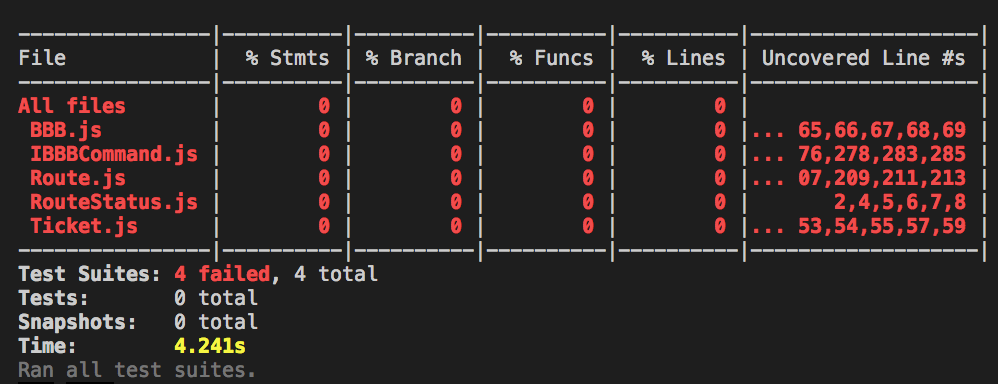
\includegraphics[width=.9\linewidth]{documentation.org.img/coverage_example.png}
\end{center}

The goal for this assignment is to reach a value of 100\% in the column \texttt{\% Branch}
for all files without any tests failing. 

\section{Notes}
\label{sec:org3de4cb7}

We found that the document was better readable when not using tables and decided to use a list formatting for better readability.
Some test cases required the targeted class to be in a certain state. Therefore, we added a \texttt{Precondition} to those test cases. For instance,
the precondition \texttt{Route\{ id: “R1”, source: "Madrid", destination: "Toledo", ...\}} means that a \texttt{Route} instance should be initialized with the 
stated properties in the arrangement of the test case. If no class name is stated at the beginning, it means that we are referring to a simple
object representation or single variables instead of a class instance. A value of \texttt{N/A} indicates that no precondition or input is required. For
shortening the definition of a list of \texttt{Tickets} we used values as for instance T1\_R1\_9 which corresponds to a \texttt{Ticket} instance on \texttt{Route} R1 
with seat 9 which is not boarded, e.g. Ticket \{ id: "T1", seat: 9, boarded: false \}.

The complete source code of the tested application is shown in the attachment.

\section{Iteration 1}
\label{sec:org5586888}

Iteration 1 targets the classes \texttt{Ticket} and \texttt{Route}

\subsection{Specify Test Cases}
\label{sec:org42fb0aa}

\subsubsection{Class Ticket}
\label{sec:org0a3f4d6}

\begin{description}
\item[{\textbf{TC\_Ticket\_1}}] initializes correctly
\begin{description}
\item[{Goal}] Test that the \texttt{Ticket} class initializes correctly
\item[{Class}] Ticket
\item[{Method}] constructor
\item[{Precondition}] N/A
\item[{Input}] \{ id: “T1”, seat: 1 \}
\item[{Expected Output}] Ticket\{ id: “T1”, seat: 1, boarded: false \}
\end{description}

\item[{\textbf{TC\_Ticket\_2}}] throws error for invalid id
\begin{description}
\item[{Goal}] Test that the \texttt{Ticket} class fails the initialization when an invalid id is passed
\item[{Class}] Ticket
\item[{Method}] constructor
\item[{Precondition}] N/A
\item[{Input}] \{ id: “ ”, seat: 1 \}
\item[{Expected Output}] Error(“Invalid id”)
\end{description}

\item[{\textbf{TC\_Ticket\_3}}] throws error for invalid seat 
\begin{description}
\item[{Goal}] Test that the \texttt{Ticket} class fails the initialization when an invalid seat number is passed
\item[{Class}] Ticket
\item[{Method}] constructor
\item[{Precondition}] N/A
\item[{Input}] \{ id: “T1”, seat: -1 \}
\item[{Expected Output}] Error(“Invalid seat”)
\end{description}

\item[{\textbf{TC\_Ticket\_4}}] changes value correctly
\begin{description}
\item[{Goal}] Test that the \texttt{boarded} property changes it's value correctly
\item[{Class}] Ticket
\item[{Method}] setter boarded
\item[{Precondition}] Ticket\{ boarded: false \}
\item[{Input}] true
\item[{Expected Output}] Ticket\{ boarded: true \}
\end{description}

\item[{\textbf{TC\_Ticket\_5}}] creates object correctly
\begin{description}
\item[{Goal}] Test that the \texttt{toObject()} method creates a correct object representation of the \texttt{Ticket}
\item[{Class}] Ticket
\item[{Method}] toObject
\item[{Precondition}] Ticket\{ id: “T1”, seat: 1, boarded: false \}
\item[{Input}] N/A
\item[{Expected Output}] Object\{id: “T1”, seat: 1, boarded: false \}
\end{description}

\item[{\textbf{TC\_Ticket\_6}}] creates ticket correctly
\begin{description}
\item[{Goal}] Test the the \texttt{fromObject()} method creates a correct \texttt{Ticket} instance from it's object representation
\item[{Class}] Ticket
\item[{Method}] fromObject
\item[{Precondition}] N/A
\item[{Input}] Object\{ id: “T1”, seat: 1, boarded: false \}
\item[{Expected Output}] Ticket\{id: “T1”, seat: 1, boarded: false \}
\end{description}

\item[{\textbf{TC\_Ticket\_7}}] throws error for invalid ticket object
\begin{description}
\item[{Goal}] Test that the \texttt{fromObject()} method throws an error if an invalid object representation is passed
\item[{Class}] Ticket
\item[{Method}] fromObject
\item[{Precondition}] N/A
\item[{Input}] Object\{ id\_X: “T1”, seat: 1, boarded: false \}
\item[{Expected Output}] Error(“Invalid object”)
\end{description}
\end{description}

\subsubsection{Class Route}
\label{sec:org74aad9b}

\begin{description}
\item[{\textbf{TC\_Route\_1}}] initializes correctly
\begin{description}
\item[{Goal}] Test that the \texttt{Route} class initializes correctly
\item[{Class}] Route
\item[{Method}] constructor
\item[{Precondition}] N/A
\item[{Input}] \{ id: “R1”, source: “Madrid”, destination: “Toledo”, capacity: 10 \}
\item[{Expected Output}] Route\{ id: “R1”, source: “Madrid”, destination: “Toledo”, capacity: 10,  tickets: [], departed: null, availableSeats: [0, … , 9]\}
\end{description}

\item[{\textbf{TC\_Route\_2}}] throws error on invalid id
\begin{description}
\item[{Goal}] Test that the \texttt{Route} class fails initialization if an invalid id is passed
\item[{Class}] Route
\item[{Method}] constructor
\item[{Precondition}] N/A
\item[{Input}] \{ id: “ ”, source: “Madrid”, destination: “Toledo”, capacity: 10 \}
\item[{Expected Output}] Error(“Invalid id”)
\end{description}

\item[{\textbf{TC\_Route\_3}}] throws error on invalid source
\begin{description}
\item[{Goal}] Test that the \texttt{Route} class fails initialization if an invalid source is given
\item[{Class}] Route
\item[{Method}] constructor
\item[{Precondition}] N/A
\item[{Input}] \{ id: “R1”, source: “ ”, destination: “Toledo”, capacity: 10 \}
\item[{Expected Output}] Error(“Invalid source”)
\end{description}

\item[{\textbf{TC\_Route\_4}}] throws error on invalid destination
\begin{description}
\item[{Goal}] Test that the \texttt{Route} class fails initialization if an invalid destination is given
\item[{Class}] Route
\item[{Method}] constructor
\item[{Precondition}] N/A
\item[{Input}] \{ id: “R1”, source: “Madrid”, destination: null, capacity: 10 \}
\item[{Expected Output}] Error(“Invalid source”)
\end{description}

\item[{\textbf{TC\_Route\_5}}] throws error on invalid capacity
\begin{description}
\item[{Goal}] Test that the \texttt{Route} class fails initialization if an invalid capacity is given
\item[{Class}] Route
\item[{Method}] constructor
\item[{Precondition}] N/A
\item[{Input}] \{ id: “R1”, source: “Madrid”, destination: “Toledo”, capacity: -1 \}
\item[{Expected Output}] Error(“Invalid capacity”)
\end{description}

\item[{\textbf{TC\_Route\_6}}] returns status “travelling” on travelling
\begin{description}
\item[{Goal}] Test that the property \texttt{status} returns "travelling" if it has departed
\item[{Class}] Route
\item[{Method}] getter status
\item[{Precondition}] Route\{ id: “R1”, source: “Madrid”, destination: “Toledo”, capacity: 10,  tickets: [], departed: “2008-09-15T15:53:00”, availableSeats: [0, … , 9]\}
\item[{Input}] N/A
\item[{Expected Output}] “travelling”
\item[{Note}] The date set for departed is an example. For the test the current date and time will be set
\end{description}

\item[{\textbf{TC\_Route\_7}}] returns status “empty” on empty
\begin{description}
\item[{Goal}] Test that the property \texttt{status} returns "empty" if it has not departed and no ticket has been purchased
\item[{Class}] Route
\item[{Method}] getter status
\item[{Precondition}] Route\{ id: “R1”, source: “Madrid”, destination: “Toledo”, capacity: 10,  tickets: [], departed: null, availableSeats: [0, … , 9]\}
\item[{Input}] N/A
\item[{Expected Output}] “empty”
\end{description}

\item[{\textbf{TC\_Route\_8}}] returns status “available” on available
\begin{description}
\item[{Goal}] Test that the property \texttt{status} returns "available" if it has not departed and at least one ticket has been purchased
\item[{Class}] Route
\item[{Method}] getter status
\item[{Precondition}] Route\{ id: “R1”, source: “Madrid”, destination: “Toledo”, capacity: 10,  tickets: [T\_R1\_9], departed: null, availableSeats: [0, … , 8]\}
\item[{Input}] N/A
\item[{Expected Output}] “available”
\end{description}

\item[{\textbf{TC\_Route\_9}}] returns status “full” on full
\begin{description}
\item[{Goal}] Test that the property \texttt{status} returns "full" if it has not departed and all available tickets have been purchased
\item[{Class}] Route
\item[{Method}] getter status
\item[{Precondition}] Route\{ id: “R1”, source: “Madrid”, destination: “Toledo”, capacity: 10,  tickets: [T\_R1\_9, …, T\_R1\_0], departed: null, availableSeats: []\}
\item[{Input}] N/A
\item[{Expected Output}] “full”
\end{description}

\item[{\textbf{TC\_Route\_10}}] successfully purchase ticket
\begin{description}
\item[{Goal}] Test that the method \texttt{purchaseTicket()} successfully creates a new \texttt{Ticket} instance and removes one available seat
\item[{Class}] Route
\item[{Method}] purchaseTicket
\item[{Precondition}] Route\{ id: “R1”, source: “Madrid”, destination: “Toledo”, capacity: 10,  tickets: [], departed: null, availableSeats: [0, …, 9]\}
\item[{Input}] N/A
\item[{Expected Output}] \{ success: true, ticket:  Ticket\{ id: “T1\_R1\_9”, seat: 9, boarded: false \} \},
Route\{ id: “R1”, source: “Madrid”, destination: “Toledo”, capacity: 10,  tickets: [T1\_R1\_9], departed: null, availableSeats: [0, …, 8]\}
\end{description}

\item[{\textbf{TC\_Route\_11}}] purchase ticket fails on no available tickets
\begin{description}
\item[{Goal}] Test that the method \texttt{purchaseTicket()} fails if there are no available seats left
\item[{Class}] Route
\item[{Method}] purchaseTicket
\item[{Precondition}] Route\{ id: “R1”, source: “Madrid”, destination: “Toledo”, capacity: 10,  tickets: [T1\_R1\_9, … T1\_R1\_0], departed: null, availableSeats: []\}
\item[{Input}] N/A
\item[{Expected Output}] \{ success: false, reason: “No tickets available” \},
Route\{ id: “R1”, source: “Madrid”, destination: “Toledo”, capacity: 10,  tickets: [T1\_R1\_9, … T1\_R1\_0], departed: null, availableSeats: []\}
\end{description}

\item[{\textbf{TC\_Route\_12}}] successfully board ticket
\begin{description}
\item[{Goal}] Test that the method \texttt{boardTicket()} successfully changes the property "boarded" of the corresponding \texttt{Ticket} to "true" and does not alter any other \texttt{Ticket}
\item[{Class}] Route
\item[{Method}] boardTicket
\item[{Precondition}] Route\{ id: “R1”, source: “Madrid”, destination: “Toledo”, capacity: 10,  tickets: [T1\_R1\_9, … T1\_R1\_0], departed: null, availableSeats: []\}, T1\_R1\_9\{ id: “T1\_R1\_9”, seat: 9, boarded: false \}
\item[{Input}] \{ ticketId: “T1\_R1\_9” \}
\item[{Expected Output}] \{ success: true, ticket:  Ticket\{ id: “T1\_R1\_9”, seat: 9, boarded: true \} \},
Route\{ id: “R1”, source: “Madrid”, destination: “Toledo”, capacity: 10,  tickets: [T1\_R1\_9, … T1\_R1\_0], departed: null, availableSeats: []\}
\end{description}

\item[{\textbf{TC\_Route\_13}}] board ticket fails for invalid ticketId
\begin{description}
\item[{Goal}] Test that the method \texttt{boardTicket()} fails if the passed \texttt{ticketId} does not match any \texttt{Ticket}
\item[{Class}] Route
\item[{Method}] boardTicket
\item[{Precondition}] Route\{ id: “R1”, source: “Madrid”, destination: “Toledo”, capacity: 10,  tickets: [T1\_R1\_9, … T1\_R1\_0], departed: null, availableSeats: []\}
\item[{Input}] \{ ticketId: “T1\_R1\_XXX” \}
\item[{Expected Output}] \{ success: false, reason: “Ticket does not exist” \},
Route\{ id: “R1”, source: “Madrid”, destination: “Toledo”, capacity: 10,  tickets: [T1\_R1\_9, … T1\_R1\_0], departed: null, availableSeats: []\}
\end{description}

\item[{\textbf{TC\_Route\_14}}] board ticket fails for already boarded ticketId
\begin{description}
\item[{Goal}] Test that the method \texttt{boardTicket()} fails if the property \texttt{boarded} of the corresponding \texttt{Ticket} is already set to true
\item[{Class}] Route
\item[{Method}] boardTicket
\item[{Precondition}] Route\{ id: “R1”, source: “Madrid”, destination: “Toledo”, capacity: 10,  tickets: [T1\_R1\_9, … T1\_R1\_0], departed: null, availableSeats: []\}, T1\_R1\_9\{ id: “T1\_R1\_9”, seat: 9, boarded: true \}
\item[{Input}] \{ ticketId: “T1\_R1\_9” \}
\item[{Expected Output}] \{ success: false, reason: “Ticket is already boarded” \},
Route\{ id: “R1”, source: “Madrid”, destination: “Toledo”, capacity: 10,  tickets: [T1\_R1\_9, … T1\_R1\_0], departed: null, availableSeats: []\}, T1\_R1\_9\{ id: “T1\_R1\_9”, seat: 9, boarded: true \}
\end{description}

\item[{\textbf{TC\_Route\_15}}] successfully cancel ticket
\begin{description}
\item[{Goal}] Test that the method \texttt{cancelTicket()} successfully removes the corresponding \texttt{Ticket} from the list of \texttt{Tickets} and adds the seat of the \texttt{Ticket} back to the list of the available seats.
\item[{Class}] Route
\item[{Method}] cancelTicket
\item[{Precondition}] Route\{ id: “R1”, source: “Madrid”, destination: “Toledo”, capacity: 10,  tickets: [T1\_R1\_9, … T1\_R1\_0], departed: null, availableSeats: []\}, T1\_R1\_9\{ id: “T1\_R1\_9”, seat: 9, boarded: false \}
\item[{Input}] \{ ticketId: “T1\_R1\_9” \}
\item[{Expected Output}] \{ success: true, ticket:  Ticket\{ id: “T1\_R1\_9”, seat: 9, boarded: false \} \},
Route\{ id: “R1”, source: “Madrid”, destination: “Toledo”, capacity: 10,  tickets: [T1\_R1\_8, … T1\_R1\_0], departed: null, availableSeats: [9]\}
\end{description}

\item[{\textbf{TC\_Route\_16}}] cancel ticket fails for invalid ticketId
\begin{description}
\item[{Goal}] Test that the method \texttt{cancelTicket()} fails if the passed \texttt{ticketId} does not match any \texttt{Ticket}
\item[{Class}] Route
\item[{Method}] cancelTicket
\item[{Precondition}] Route\{ id: “R1”, source: “Madrid”, destination: “Toledo”, capacity: 10,  tickets: [T1\_R1\_9, … T1\_R1\_0], departed: null, availableSeats: []\}
\item[{Input}] \{ ticketId: “T1\_R1\_XXX” \}
\item[{Expected Output}] \{ success: false, reason: “Ticket does not exist” \},
Route\{ id: “R1”, source: “Madrid”, destination: “Toledo”, capacity: 10,  tickets: [T1\_R1\_9, … T1\_R1\_0], departed: null, availableSeats: []\}
\end{description}

\item[{\textbf{TC\_Route\_17}}] cancel ticket fails for already boarded ticketId
\begin{description}
\item[{Goal}] Test that the method \texttt{cancelTicket()} fails if the property \texttt{boarded} of the corresponding \texttt{Ticket} is already set to true
\item[{Class}] Route
\item[{Method}] cancelTicket
\item[{Precondition}] Route\{ id: “R1”, source: “Madrid”, destination: “Toledo”, capacity: 10,  tickets: [T1\_R1\_9, … T1\_R1\_0], departed: null, availableSeats: []\}, T1\_R1\_9\{ id: “T1\_R1\_9”, seat: 9, boarded: true \}
\item[{Input}] \{ ticketId: “T1\_R1\_9” \}
\item[{Expected Output}] \{ success: false, reason: “Ticket is already boarded” \},
Route\{ id: “R1”, source: “Madrid”, destination: “Toledo”, capacity: 10,  tickets: [T1\_R1\_9, … T1\_R1\_0], departed: null, availableSeats: []\}, T1\_R1\_9\{ id: “T1\_R1\_9”, seat: 9, boarded: true \}
\end{description}

\item[{\textbf{TC\_Route\_18}}] depart successfully sets departure time
\begin{description}
\item[{Goal}] Test that the method \texttt{depart()} successfully sets the departure of the \texttt{Route} with a current timestamp
\item[{Class}] Route
\item[{Method}] depart
\item[{Precondition}] Route\{ id: “R1”, source: “Madrid”, destination: “Toledo”, capacity: 10,  tickets: [], departed: null, availableSeats: [0, …, 9]\}
\item[{Input}] N/A
\item[{Expected Output}] Route\{ id: “R1”, source: “Madrid”, destination: “Toledo”, capacity: 10,  tickets: [], departed: “2008-09-15T15:53:00”, availableSeats: [0, …, 9]\}
\item[{Note}] The date set for departed is an example. For the test the current date and time will be set
\end{description}

\item[{\textbf{TC\_Route\_19}}] hasArrived successfully resets the Route
\begin{description}
\item[{Goal}] Test that the method \texttt{hasArrived()} successfully resets the departure to null if the departure is set and at least 10 seconds have been passed since the departure
\item[{Class}] Route
\item[{Method}] hasArrived
\item[{Precondition}] Route\{ id: “R1”, source: “Madrid”, destination: “Toledo”, capacity: 10,  tickets: [T1\_R1\_9, … T1\_R1\_0], departed: “2008-09-15T15:53:00”, availableSeats: []\}
\item[{Input}] N/A
\item[{Expected Output}] true, Route\{ id: “R1”, source: “Toledo”, destination: “Madrid”, capacity: 10,  tickets: [], departed: null, availableSeats: [0, …, 9]\}
\item[{Note}] The date set for departed is an example. For the test the current date and time will be set
\end{description}

\item[{\textbf{TC\_Route\_20}}] hasArrived does not reset the Route if no departed yet
\begin{description}
\item[{Goal}] Test that the method \texttt{hasArrived()} does nothing if no departure is set
\item[{Class}] Route
\item[{Method}] hasArrived
\item[{Precondition}] Route\{ id: “R1”, source: “Madrid”, destination: “Toledo”, capacity: 10,  tickets: [T1\_R1\_9, … T1\_R1\_0], departed: null, availableSeats: []\}
\item[{Input}] N/A
\item[{Expected Output}] false, Route\{ id: “R1”, source: “Madrid”, destination: “Toledo”, capacity: 10,  tickets: [T1\_R1\_9, … T1\_R1\_0], departed: null, availableSeats: []\}
\end{description}

\item[{\textbf{TC\_Route\_21}}] hasArrived does not reset the Route if still travelling
\begin{description}
\item[{Goal}] Test that the method \texttt{hasArrived()} does nothing if the departure is set but less than 10 seconds have been passed since departure
\item[{Class}] Route
\item[{Method}] hasArrived
\item[{Precondition}] Route\{ id: “R1”, source: “Madrid”, destination: “Toledo”, capacity: 10,  tickets: [T1\_R1\_9, … T1\_R1\_0], departed: “2008-09-15T15:53:00”, availableSeats: []\}
\item[{Input}] N/A
\item[{Expected Output}] false, Route\{ id: “R1”, source: “Madrid”, destination: “Toledo”, capacity: 10,  tickets: [T1\_R1\_9, … T1\_R1\_0], departed: “2008-09-15T15:53:00”, availableSeats: []\}
\item[{Note}] The date set for departed is an example. For the test the current date and time will be set so that the 10 seconds have not passed yet
\end{description}

\item[{\textbf{TC\_Route\_22}}] fromObject successfully creates new Route with set departure
\begin{description}
\item[{Goal}] Test that the \texttt{fromObject()} method successfully creates a \texttt{Route} instance from it's object representation that has a departure set
\item[{Class}] Route
\item[{Method}] fromObject
\item[{Precondition}] N/A
\item[{Input}] \{ id: “R1”, source: “Madrid”, destination: “Toledo”, capacity: 10,  tickets: [T1\_R1\_9, … T1\_R1\_3], departed: “2008-09-15T15:53:00”, availableSeats: [0, 1, 2]\}
\item[{Expected Output}] Route\{ id: “R1”, source: “Madrid”, destination: “Toledo”, capacity: 10,  tickets: [T1\_R1\_9, … T1\_R1\_3], departed: “2008-09-15T15:53:00”, availableSeats: [0, 1, 2]\}
\item[{Note}] The date set for departed is an example
\end{description}

\item[{\textbf{TC\_Route\_23}}] fromObject successfully creates new Route without set departure and tickets
\begin{description}
\item[{Goal}] Test that the \texttt{fromObject()} method successfully creates a \texttt{Route} instance from it's object representation that does not have a departure set
\item[{Class}] Route
\item[{Method}] fromObject
\item[{Precondition}] N/A
\item[{Input}] \{ id: “R1”, source: “Madrid”, destination: “Toledo”, capacity: 10,  tickets: [], departed: null, availableSeats: [0, …, 9]\}
\item[{Expected Output}] Route\{ id: “R1”, source: “Madrid”, destination: “Toledo”, capacity: 10,  tickets: [], departed: null, availableSeats: [0, …, 9]\}
\end{description}

\item[{\textbf{TC\_Route\_24}}] toObject successfully creates new Object with set departure
\begin{description}
\item[{Goal}] Test that the \texttt{toObject()} method successfully creates a object representation of the \texttt{Route} that has a departure set
\item[{Class}] Route
\item[{Method}] toObject
\item[{Precondition}] Route\{ id: “R1”, source: “Madrid”, destination: “Toledo”, capacity: 10,  tickets: [T1\_R1\_9, … T1\_R1\_3], departed: “2008-09-15T15:53:00”, availableSeats: [0, 1, 2]\}
\item[{Input}] N/A
\item[{Expected Output}] Object\{ id: “R1”, source: “Madrid”, destination: “Toledo”, capacity: 10,  tickets: [T1\_R1\_9, … T1\_R1\_3], departed: “2008-09-15T15:53:00”, availableSeats: [0, 1, 2]\}
\end{description}

\item[{\textbf{TC\_Route\_25}}] toObject successfully creates new Object without departure
\begin{description}
\item[{Goal}] Test that the \texttt{toObject()} method successfully creates a object representation of the \texttt{Route} that does not have a departure set
\item[{Class}] Route
\item[{Method}] toObject
\item[{Precondition}] Route\{ id: “R1”, source: “Madrid”, destination: “Toledo”, capacity: 10,  tickets: [T1\_R1\_9, … T1\_R1\_3], departed: null, availableSeats: [0, 1, 2]\}
\item[{Input}] N/A
\item[{Expected Output}] Object\{ id: “R1”, source: “Madrid”, destination: “Toledo”, capacity: 10,  tickets: [T1\_R1\_9, … T1\_R1\_3], departed: null, availableSeats: [0, 1, 2]\}
\end{description}
\end{description}

\subsection{Run Test Cases}
\label{sec:org3ad1a0b}

\subsubsection{Class Ticket}
\label{sec:orgc7613fe}

\begin{itemize}
\item \textbf{TC\_Ticket\_1}
\begin{description}
\item[{Expected Output}] Ticket\{ id: “T1”, seat: 1, boarded: false \}
\item[{Observed Output}] Ticket\{ id: “T1”, seat: 1, boarded: false \}
\item[{Failure}] None
\end{description}

\item \textbf{TC\_Ticket\_2}
\begin{description}
\item[{Expected Output}] Error(“Invalid id”)
\item[{Observed Output}] Error(“Invalid id”)
\item[{Failure}] None
\end{description}

\item \textbf{TC\_Ticket\_3}
\begin{description}
\item[{Expected Output}] Error(“Invalid seat”)
\item[{Observed Output}] Error(“Invalid seat”)
\item[{Failure}] None
\end{description}

\item \textbf{TC\_Ticket\_4}
\begin{description}
\item[{Expected Output}] Ticket\{ boarded: true \}
\item[{Observed Output}] Ticket\{ boarded: true \}
\item[{Failure}] None
\end{description}

\item \textbf{TC\_Ticket\_5}
\begin{description}
\item[{Expected Output}] Object\{id: “T1”, seat: 1, boarded: false \}
\item[{Observed Output}] Object\{id: “T1”, seat: 1, boarded: false \}
\item[{Failure}] None
\end{description}

\item \textbf{TC\_Ticket\_6}
\begin{description}
\item[{Expected Output}] Ticket\{id: “T1”, seat: 1, boarded: false \}
\item[{Observed Output}] Ticket\{id: “T1”, seat: 1, boarded: false \}
\item[{Failure}] None
\end{description}

\item \textbf{TC\_Ticket\_7}
\begin{description}
\item[{Expected Output}] Error(“Invalid object”)
\item[{Observed Output}] Error(“Invalid object”)
\item[{Failure}] None
\end{description}
\end{itemize}

\subsubsection{Class Route}
\label{sec:org1865968}

\begin{itemize}
\item \textbf{TC\_Route\_1}
\begin{description}
\item[{Expected Output}] Route\{ id: “R1”, source: “Madrid”, destination: “Toledo”, capacity: 10,  tickets: [], departed: null, availableSeats: [0, … , 9]\}
\item[{Observed Output}] Route\{ id: “R1”, source: “Madrid”, destination: “Toledo”, capacity: 10,  tickets: [], departed: null, availableSeats: [0, … , 9]\}
\item[{Failure}] None
\end{description}

\item \textbf{TC\_Route\_2}
\begin{description}
\item[{Expected Output}] Error(“Invalid id”)
\item[{Observed Output}] Error(“Invalid id”)
\item[{Failure}] None
\end{description}

\item \textbf{TC\_Route\_3}
\begin{description}
\item[{Expected Output}] Error(“Invalid source”)
\item[{Observed Output}] Error(“Invalid source”)
\item[{Failure}] None
\end{description}

\item \textbf{TC\_Route\_4}
\begin{description}
\item[{Expected Output}] Error(“Invalid source”)
\item[{Observed Output}] Error(“Invalid source”)
\item[{Failure}] None
\end{description}

\item \textbf{TC\_Route\_5}
\begin{description}
\item[{Expected Output}] Error(“Invalid capacity”)
\item[{Observed Output}] Error(“Invalid capacity”)
\item[{Failure}] None
\end{description}

\item \textbf{TC\_Route\_6}
\begin{description}
\item[{Expected Output}] “travelling”
\item[{Observed Output}] 0
\item[{Failure}] Yes
\end{description}

\item \textbf{TC\_Route\_7}
\begin{description}
\item[{Expected Output}] “empty”
\item[{Observed Output}] 1
\item[{Failure}] Yes
\end{description}

\item \textbf{TC\_Route\_8}
\begin{description}
\item[{Expected Output}] “available”
\item[{Observed Output}] 3
\item[{Failure}] Yes
\end{description}

\item \textbf{TC\_Route\_9}
\begin{description}
\item[{Expected Output}] “full”
\item[{Observed Output}] 2
\item[{Failure}] Yes
\end{description}

\item \textbf{TC\_Route\_10}
\begin{description}
\item[{Expected Output}] \{ success: true, ticket:  Ticket\{ id: “T1\_R1\_9”, seat: 9, boarded: false \} \},
Route\{ id: “R1”, source: “Madrid”, destination: “Toledo”, capacity: 10,  tickets: [T1\_R1\_9], departed: null, availableSeats: [0, …, 8]\}
\item[{Observed Output}] \{ success: true, ticket:  Ticket\{ id: “T1\_R1\_9”, seat: 9, boarded: false \} \},
Route\{ id: “R1”, source: “Madrid”, destination: “Toledo”, capacity: 10,  tickets: [T1\_R1\_9], departed: null, availableSeats: [0, …, 8]\}
\item[{Failure}] None
\end{description}

\item \textbf{TC\_Route\_11}
\begin{description}
\item[{Expected Output}] \{ success: false, reason: “No tickets available” \},
Route\{ id: “R1”, source: “Madrid”, destination: “Toledo”, capacity: 10,  tickets: [T1\_R1\_9, … T1\_R1\_0], departed: null, availableSeats: []\}
\item[{Observed Output}] \{ success: false, reason: “No tickets available” \},
Route\{ id: “R1”, source: “Madrid”, destination: “Toledo”, capacity: 10,  tickets: [T1\_R1\_9, … T1\_R1\_0], departed: null, availableSeats: []\}
\item[{Failure}] None
\end{description}

\item \textbf{TC\_Route\_12}
\begin{description}
\item[{Expected Output}] \{ success: true, ticket:  Ticket\{ id: “T1\_R1\_9”, seat: 9, boarded: true \} \},
Route\{ id: “R1”, source: “Madrid”, destination: “Toledo”, capacity: 10,  tickets: [T1\_R1\_9, … T1\_R1\_0], departed: null, availableSeats: []\}
\item[{Observed Output}] \{ success: true, ticket:  Ticket\{ id: “T1\_R1\_9”, seat: 9, boarded: true \} \},
Route\{ id: “R1”, source: “Madrid”, destination: “Toledo”, capacity: 10,  tickets: [T1\_R1\_9, … T1\_R1\_0], departed: null, availableSeats: []\}
\item[{Failure}] None
\end{description}

\item \textbf{TC\_Route\_13}
\begin{description}
\item[{Expected Output}] \{ success: false, reason: “Ticket does not exist” \},
Route\{ id: “R1”, source: “Madrid”, destination: “Toledo”, capacity: 10,  tickets: [T1\_R1\_9, … T1\_R1\_0], departed: null, availableSeats: []\}
\item[{Observed Output}] \{ success: false, reason: “Ticket does not exist” \},
Route\{ id: “R1”, source: “Madrid”, destination: “Toledo”, capacity: 10,  tickets: [T1\_R1\_9, … T1\_R1\_0], departed: null, availableSeats: []\}
\item[{Failure}] None
\end{description}

\item \textbf{TC\_Route\_14}
\begin{description}
\item[{Expected Output}] \{ success: false, reason: “Ticket is already boarded” \},
Route\{ id: “R1”, source: “Madrid”, destination: “Toledo”, capacity: 10,  tickets: [T1\_R1\_9, … T1\_R1\_0], departed: null, availableSeats: []\}, T1\_R1\_9\{ id: “T1\_R1\_9”, seat: 9, boarded: true \}
\item[{Observed Output}] \{ success: false, reason: “Ticket is already boarded” \},
Route\{ id: “R1”, source: “Madrid”, destination: “Toledo”, capacity: 10,  tickets: [T1\_R1\_9, … T1\_R1\_0], departed: null, availableSeats: []\}, T1\_R1\_9\{ id: “T1\_R1\_9”, seat: 9, boarded: true \}
\item[{Failure}] None
\end{description}

\item \textbf{TC\_Route\_15}
\begin{description}
\item[{Expected Output}] \{ success: true, ticket:  Ticket\{ id: “T1\_R1\_9”, seat: 9, boarded: false \} \},
Route\{ id: “R1”, source: “Madrid”, destination: “Toledo”, capacity: 10,  tickets: [T1\_R1\_8, … T1\_R1\_0], departed: null, availableSeats: [9]\}
\item[{Observed Output}] \{ success: true, ticket:  Ticket\{ id: “T1\_R1\_9”, seat: 9, boarded: false \} \},
Route\{ id: “R1”, source: “Madrid”, destination: “Toledo”, capacity: 10,  tickets: [T1\_R1\_8, … T1\_R1\_0], departed: null, availableSeats: []\}
\item[{Failure}] Yes
\end{description}

\item \textbf{TC\_Route\_16}
\begin{description}
\item[{Expected Output}] \{ success: false, reason: “Ticket does not exist” \},
Route\{ id: “R1”, source: “Madrid”, destination: “Toledo”, capacity: 10,  tickets: [T1\_R1\_9, … T1\_R1\_0], departed: null, availableSeats: []\}
\item[{Observed Output}] \{ success: false, reason: “Ticket does not exist” \},
Route\{ id: “R1”, source: “Madrid”, destination: “Toledo”, capacity: 10,  tickets: [T1\_R1\_9, … T1\_R1\_0], departed: null, availableSeats: []\}
\item[{Failure}] None
\end{description}

\item \textbf{TC\_Route\_17}
\begin{description}
\item[{Expected Output}] \{ success: false, reason: “Ticket is already boarded” \},
Route\{ id: “R1”, source: “Madrid”, destination: “Toledo”, capacity: 10,  tickets: [T1\_R1\_9, … T1\_R1\_0], departed: null, availableSeats: []\}, T1\_R1\_9\{ id: “T1\_R1\_9”, seat: 9, boarded: true \}
\item[{Observed Output}] \{ success: false, reason: “Ticket is already boarded” \},
Route\{ id: “R1”, source: “Madrid”, destination: “Toledo”, capacity: 10,  tickets: [T1\_R1\_9, … T1\_R1\_0], departed: null, availableSeats: []\}, T1\_R1\_9\{ id: “T1\_R1\_9”, seat: 9, boarded: true \}
\item[{Failure}] None
\end{description}

\item \textbf{TC\_Route\_18}
\begin{description}
\item[{Expected Output}] Route\{ id: “R1”, source: “Madrid”, destination: “Toledo”, capacity: 10,  tickets: [], departed: “2008-09-15T15:53:00”, availableSeats: [0, …, 9]\}
\item[{Observed Output}] Route\{ id: “R1”, source: “Madrid”, destination: “Toledo”, capacity: 10,  tickets: [], departed: “2008-09-15T15:53:00”, availableSeats: [0, …, 9]\}
\item[{Failure}] None
\end{description}

\item \textbf{TC\_Route\_19}
\begin{description}
\item[{Expected Output}] true, Route\{ id: “R1”, source: “Toledo”, destination: “Madrid”, capacity: 10,  tickets: [], departed: null, availableSeats: [0, …, 9]\}
\item[{Observed Output}] true, Route\{ id: “R1”, source: “Toledo”, destination: “Madrid”, capacity: 10,  tickets: [], departed: null, availableSeats: [0, …, 9]\}
\item[{Failure}] None
\end{description}

\item \textbf{TC\_Route\_20}
\begin{description}
\item[{Expected Output}] false, Route\{ id: “R1”, source: “Madrid”, destination: “Toledo”, capacity: 10,  tickets: [T1\_R1\_9, … T1\_R1\_0], departed: null, availableSeats: []\}
\item[{Observed Output}] false, Route\{ id: “R1”, source: “Madrid”, destination: “Toledo”, capacity: 10,  tickets: [T1\_R1\_9, … T1\_R1\_0], departed: null, availableSeats: []\}
\item[{Failure}] None
\end{description}

\item \textbf{TC\_Route\_21}
\begin{description}
\item[{Expected Output}] false, Route\{ id: “R1”, source: “Madrid”, destination: “Toledo”, capacity: 10,  tickets: [T1\_R1\_9, … T1\_R1\_0], departed: “2008-09-15T15:53:00”, availableSeats: []\}
\item[{Observed Output}] false, Route\{ id: “R1”, source: “Madrid”, destination: “Toledo”, capacity: 10,  tickets: [T1\_R1\_9, … T1\_R1\_0], departed: “2008-09-15T15:53:00”, availableSeats: []\}
\item[{Failure}] None
\end{description}

\item \textbf{TC\_Route\_22}
\begin{description}
\item[{Expected Output}] Route\{ id: “R1”, source: “Madrid”, destination: “Toledo”, capacity: 10,  tickets: [T1\_R1\_9, … T1\_R1\_3], departed: “2008-09-15T15:53:00”, availableSeats: [0, 1, 2]\}
\item[{Observed Output}] Route\{ id: “R1”, source: “Madrid”, destination: “Toledo”, capacity: 10,  tickets: [T1\_R1\_9, … T1\_R1\_3], departed: “2008-09-15T15:53:00”, availableSeats: [0, 1, 2]\}
\item[{Failure}] None
\end{description}

\item \textbf{TC\_Route\_23}
\begin{description}
\item[{Expected Output}] Route\{ id: “R1”, source: “Madrid”, destination: “Toledo”, capacity: 10,  tickets: [], departed: null, availableSeats: [0, …, 9]\}
\item[{Observed Output}] Route\{ id: “R1”, source: “Madrid”, destination: “Toledo”, capacity: 10,  tickets: [], departed: null, availableSeats: [0, …, 9]\}
\item[{Failure}] None
\end{description}

\item \textbf{TC\_Route\_24}
\begin{description}
\item[{Expected Output}] Object\{ id: “R1”, source: “Madrid”, destination: “Toledo”, capacity: 10,  tickets: [T1\_R1\_9, … T1\_R1\_3], departed: “2008-09-15T15:53:00”, availableSeats: [0, 1, 2]\}
\item[{Observed Output}] Object\{ id: “R1”, source: “Madrid”, destination: “Toledo”, capacity: 10,  tickets: [T1\_R1\_9, … T1\_R1\_3], departed: “2008-09-15T15:53:00”, availableSeats: [0, 1, 2]\}
\item[{Failure}] None
\end{description}

\item \textbf{TC\_Route\_25}
\begin{description}
\item[{Expected Output}] Object\{ id: “R1”, source: “Madrid”, destination: “Toledo”, capacity: 10,  tickets: [T1\_R1\_9, … T1\_R1\_3], departed: null, availableSeats: [0, 1, 2]\}
\item[{Observed Output}] Object\{ id: “R1”, source: “Madrid”, destination: “Toledo”, capacity: 10,  tickets: [T1\_R1\_9, … T1\_R1\_3], departed: null, availableSeats: [0, 1, 2]\}
\item[{Failure}] None
\end{description}
\end{itemize}

\subsection{Check Coverage}
\label{sec:org90fa7be}

\begin{center}
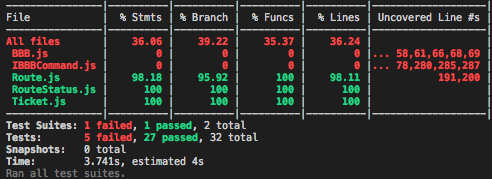
\includegraphics[width=.9\linewidth]{./Iteration2.rtfd/Pasted Graphic 1.tiff.png}
\end{center}


Using the coverage tool we identified following lines/branches not covered (red line means the line was not executed, "I" indicates that the "if" path was never taken). 
The test cases covering those lines will be added in iteration 2. 

\begin{center}
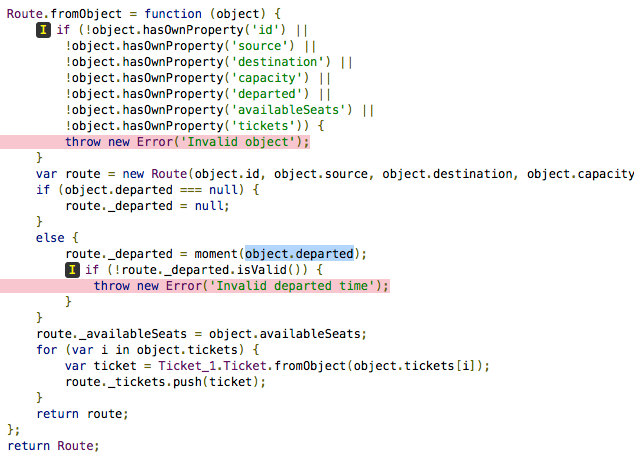
\includegraphics[width=.9\linewidth]{documentation.org.img/Iteration1_Missing_TC.png}
\end{center}


\subsection{Trace failures to faults}
\label{sec:orga397522}

\subsubsection{TC\_Route\_6, TC\_Route\_7, TC\_Route\_8, TC\_Route\_9}
\label{sec:org7f662be}

\begin{description}
\item[{Failure}] The output of the \texttt{status} property of the \texttt{Route} class returns an \texttt{int} value instead of a meaningful \texttt{string} value
\item[{Fault}] The \texttt{RouteStatus} enumeration uses \texttt{int} representation (default behavior) instead of \texttt{string} representations
\begin{center}
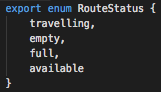
\includegraphics[width=.9\linewidth]{./Iteration2.rtfd/Pasted Graphic 4.tiff.png}
\end{center}
\item[{Fix}] Assign \texttt{string} values to \texttt{RouteStatus} enumeration:
\begin{center}
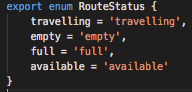
\includegraphics[width=.9\linewidth]{./Iteration2.rtfd/Pasted Graphic 5.tiff.png}
\end{center}
\end{description}

\subsubsection{TC\_Route\_15}
\label{sec:org337cb0f}

\begin{description}
\item[{Failure}] When cancelling a \texttt{Ticket} the seat that is available again is not added again to the list of available seats
\item[{Fault}] The \texttt{cancelTicket()} method misses the necessary statements that push the seat of the cancelled \texttt{Ticket} back onto the \texttt{availableSeats} list
\begin{center}
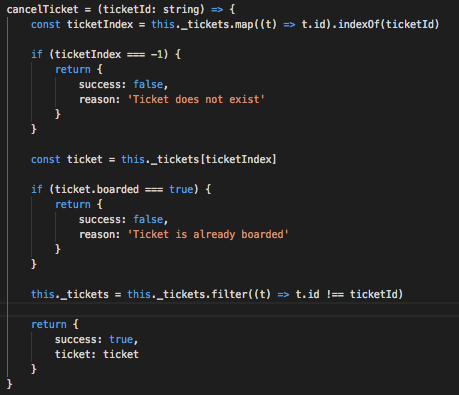
\includegraphics[width=.9\linewidth]{./Iteration2.rtfd/Pasted Graphic 2.tiff.png}
\end{center}
\item[{Fix}] Added the seat of the ticket to the list of available seats:
\begin{center}
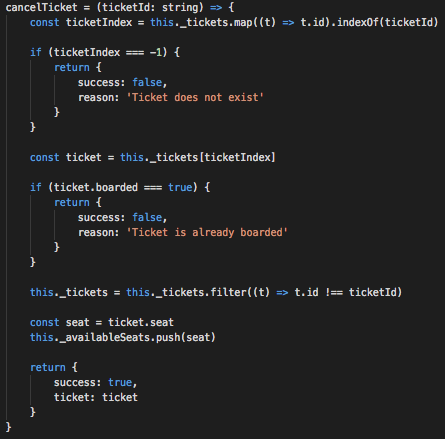
\includegraphics[width=.9\linewidth]{./Iteration2.rtfd/1_Pasted Graphic 3.tiff.png}
\end{center}
\end{description}

\section{Iteration 2}
\label{sec:org1440b24}

Iteration 2 first specifies the test cases that were identified missing from iteration 1. Then \texttt{IBBBCommand} and \texttt{BBB} are targeted.

\subsection{Specify Test Cases}
\label{sec:org25bcdb5}

\subsubsection{Class Route (Identified to be missing in last iteration)}
\label{sec:orgf850004}

\begin{description}
\item[{TC\_Route\_26}] fromObject fails on invalid object
\begin{description}
\item[{Goal}] Test that the \texttt{fromObject()} method throws an error if an invalid object representation is passed
\item[{Class}] Route
\item[{Method}] fromObject
\item[{Precondition}] N/A
\item[{Input}] \{ id\_X: “R1”, source: “Madrid”, destination: “Toledo”, capacity: 10,  tickets: [], departed: null, availableSeats: [0, 1, 2, 3, 4, 5, 6, 7, 8, 9]\}
\item[{Expected Output}] Error(‘Invalid object’)
\item[{Note}] The date set for departed is an example
\end{description}

\item[{TC\_Route\_27}] fromObject fails on invalid departure time
\begin{description}
\item[{Goal}] Test that the \texttt{fromObject()} method throws an error if departed is set to an invalid value
\item[{Class}] Route
\item[{Method}] fromObject
\item[{Precondition}] N/A
\item[{Input}] \{ id: “R1”, source: “Madrid”, destination: “Toledo”, capacity: 10,  tickets: [], departed: “4711”, availableSeats: [0, 1, 2, 3, 4, 5, 6, 7, 8, 9]\}
\item[{Expected Output}] Error(‘Invalid departed time’)
\end{description}
\end{description}

\subsubsection{Class IBBBCommand}
\label{sec:org6b86719}

\begin{description}
\item[{TC\_RegisterRouteCommand\_1}] returns correct id
\begin{description}
\item[{Goal}] Test that the \texttt{commandId} of the \texttt{RegisterRouteCommand} returns the correct value
\item[{Class}] RegisterRouteCommand
\item[{Method}] commandId get
\item[{Precondition}] N/A
\item[{Input}] N/A
\item[{Expected Output}] ‘registerroute’
\end{description}

\item[{TC\_RegisterRouteCommand\_2}] fails for invalid number of arguments
\begin{description}
\item[{Goal}] Test that the \texttt{RegisterRouteCommand} displays the correct error message if an invalid number of arguments is given
\item[{Class}] RegisterRouteCommand
\item[{Method}] execute
\item[{Precondition}] BBB\{ \_routes: [] \}
\item[{Input}] []
\item[{Expected Output}] BBB\{ \_routes: [] \}
Console: ’Invalid number of arguments given’
\end{description}

\item[{TC\_RegisterRouteCommand\_3}] fails for invalid route
\begin{description}
\item[{Goal}] Test that the \texttt{RegisterRouteCommand} displays the correct error message if an invalid value for route is given
\item[{Class}] RegisterRouteCommand
\item[{Method}] execute
\item[{Precondition}] BBB\{ \_routes: [] \}
\item[{Input}] [“ ”, “Madrid”, “Toledo”, 10]
\item[{Expected Output}] BBB\{ \_routes: [] \}
Console: ‘Invalid value for route given’
\end{description}

\item[{TC\_RegisterRouteCommand\_4}] fails for invalid source
\begin{description}
\item[{Goal}] Test that the \texttt{RegisterRouteCommand} displays the correct error message if an invalid value for source is given
\item[{Class}] RegisterRouteCommand
\item[{Method}] execute
\item[{Precondition}] BBB\{ \_routes: [] \}
\item[{Input}] [“R1”, null, “Toledo”, 10]
\item[{Expected Output}] BBB\{ \_routes: [] \}
Console: ‘Invalid value for source given’
\end{description}

\item[{TC\_RegisterRouteCommand\_5}] fails for invalid destination
\begin{description}
\item[{Goal}] Test that the \texttt{RegisterRouteCommand} displays the correct error message if an invalid destination is given
\item[{Class}] RegisterRouteCommand
\item[{Method}] execute
\item[{Precondition}] BBB\{ \_routes: [] \}
\item[{Input}] [“R1”, “Madrid”, undefined, 10]
\item[{Expected Output}] BBB\{ \_routes: [] \}
Console: ‘Invalid value for destination given’
\end{description}

\item[{TC\_RegisterRouteCommand\_6}] fails for invalid capacity
\begin{description}
\item[{Goal}] Test that the \texttt{RegisterRouteCommand} displays the correct error message if an invalid capacity is given
\item[{Class}] RegisterRouteCommand
\item[{Method}] execute
\item[{Precondition}] BBB\{ \_routes: [] \}
\item[{Input}] [“R1”, “Madrid”, “Toledo”, “asdf”]
\item[{Expected Output}] BBB\{ \_routes: [] \}
Console: ‘Invalid value for capacity’
\end{description}

\item[{TC\_RegisterRouteCommand\_7}] succeeds for valid input
\begin{description}
\item[{Goal}] Test that the \texttt{RegisterRouteCommand} successfully registers a new \texttt{Route}
\item[{Class}] RegisterRouteCommand
\item[{Method}] execute
\item[{Precondition}] BBB\{ \_routes: [] \}
\item[{Input}] [“R1”, “Madrid”, “Toledo”, 10”]
\item[{Expected Output}] BBB\{ \_routes: [Route\{ id: “R1”, source: “Madrid”, destination: “Toledo”, capacity: 10,  tickets: [], departed: null, availableSeats: [0, … , 9]\}]\}
Console: “Created route R1 from Madrid to Toledo with 10 seats”
\end{description}

\item[{TC\_DeleteRouteCommand\_1}] returns correct id
\begin{description}
\item[{Goal}] Test that the \texttt{commandId} of the "DeleteRouteCommand" returns the correct value
\item[{Class}] DeleteRouteCommand
\item[{Method}] commandId get
\item[{Precondition}] N/A
\item[{Input}] N/A
\item[{Expected Output}] ‘deleteroute’
\end{description}

\item[{TC\_DeleteRouteCommand\_2}] fails for invalid number of arguments
\begin{description}
\item[{Goal}] Test that the \texttt{DeleteRouteCommand} displays the correct error message if an invalid number of arguments is given
\item[{Class}] DeleteRouteCommand
\item[{Method}] execute
\item[{Precondition}] BBB\{ \_routes: [Route\{ id: “R1”, source: “Madrid”, destination: “Toledo”, capacity: 10,  tickets: [T\_R1\_9], departed: null, availableSeats: [0, … , 8]\}]\}
\item[{Input}] []
\item[{Expected Output}] BBB\{ \_routes: [Route\{ id: “R1”, source: “Madrid”, destination: “Toledo”, capacity: 10,  tickets: [T\_R1\_9], departed: null, availableSeats: [0, … , 8]\}]\}
Console: ‘Invalid number of arguments given’
\end{description}

\item[{TC\_DeleteRouteCommand\_3}] fails for invalid route
\begin{description}
\item[{Goal}] Test that the \texttt{DeleteRouteCommand} displays the correct error message if an invalid value for route is given
\item[{Class}] DeleteRouteCommand
\item[{Method}] execute
\item[{Precondition}] BBB\{ \_routes: [Route\{ id: “R1”, source: “Madrid”, destination: “Toledo”, capacity: 10,  tickets: [T\_R1\_9], departed: null, availableSeats: [0, … , 8]\}]\}
\item[{Input}] [“ ”]
\item[{Expected Output}] BBB\{ \_routes: [Route\{ id: “R1”, source: “Madrid”, destination: “Toledo”, capacity: 10,  tickets: [T\_R1\_9], departed: null, availableSeats: [0, … , 8]\}]\}
Console: ‘Invalid value for route given’
\end{description}

\item[{TC\_DeleteRouteCommand\_4}] fails for route with purchased tickets
\begin{description}
\item[{Goal}] Test that the \texttt{DeleteRouteCommand} does not delete a \texttt{Route} that includes already purchased \texttt{Tickets}
\item[{Class}] DeleteRouteCommand
\item[{Method}] execute
\item[{Precondition}] BBB\{ \_routes: [Route\{ id: “R1”, source: “Madrid”, destination: “Toledo”, capacity: 10,  tickets: [T\_R1\_9], departed: null, availableSeats: [0, … , 8]\}]\}
\item[{Input}] [“R1”]
\item[{Expected Output}] BBB\{ \_routes: [Route\{ id: “R1”, source: “Madrid”, destination: “Toledo”, capacity: 10,  tickets: [T\_R1\_9], departed: null, availableSeats: [0, … , 8]\}]\}
Console: “Cannot delete route R1 because there are 1 tickets booked”
\end{description}

\item[{TC\_DeleteRouteCommand\_5}] succeeds for valid input
\begin{description}
\item[{Goal}] Test that the \texttt{DeleteRouteCommand} successfully deletes a \texttt{Route} that has no purchased \texttt{Tickets}
\item[{Class}] DeleteRouteCommand
\item[{Method}] execute
\item[{Precondition}] BBB\{ \_routes: [Route\{ id: “R1”, source: “Madrid”, destination: “Toledo”, capacity: 10,  tickets: [], departed: null, availableSeats: [0, … , 9]\}]\}
\item[{Input}] [“R1”]
\item[{Expected Output}] BBB\{ \_routes: [] \}
Console: “Successfully deleted route R1”
\end{description}

\item[{TC\_DepartCommand\_1}] returns correct id
\begin{description}
\item[{Goal}] Test that the \texttt{commandId} of the "DepartCommand" returns the correct value
\item[{Class}] DepartCommand
\item[{Method}] commandId get
\item[{Precondition}] N/A
\item[{Input}] N/A
\item[{Expected Output}] ‘depart’
\end{description}

\item[{TC\_DepartCommand\_2}] fails for invalid number of arguments
\begin{description}
\item[{Goal}] Test that the \texttt{DepartCommand} displays the correct error message if an invalid number of arguments is given
\item[{Class}] DepartCommand
\item[{Method}] execute
\item[{Precondition}] BBB\{ \_routes: [Route\{ id: “R1”, source: “Madrid”, destination: “Toledo”, capacity: 10,  tickets: [T\_R1\_9], departed: null, availableSeats: [0, … , 8]\}]\}
\item[{Input}] []
\item[{Expected Output}] BBB\{ \_routes: [Route\{ id: “R1”, source: “Madrid”, destination: “Toledo”, capacity: 10,  tickets: [T\_R1\_9], departed: null, availableSeats: [0, … , 8]\}]\}
Console: ‘Invalid number of arguments given’
\end{description}

\item[{TC\_DepartCommand\_3}] fails for invalid route
\begin{description}
\item[{Goal}] Test that the \texttt{DepartCommand} displays the correct error message if an invalid value for route is given
\item[{Class}] DepartCommand
\item[{Method}] execute
\item[{Precondition}] BBB\{ \_routes: [Route\{ id: “R1”, source: “Madrid”, destination: “Toledo”, capacity: 10,  tickets: [T\_R1\_9], departed: null, availableSeats: [0, … , 8]\}]\}
\item[{Input}] [“R\_X”]
\item[{Expected Output}] BBB\{ \_routes: [Route\{ id: “R1”, source: “Madrid”, destination: “Toledo”, capacity: 10,  tickets: [T\_R1\_9], departed: null, availableSeats: [0, … , 8]\}]\}
Console: ‘Invalid value for route given’
\end{description}

\item[{TC\_DepartCommand\_4}] succeeds for valid route
\begin{description}
\item[{Goal}] Test that the \texttt{DepartCommand} successfully sets the departure of a \texttt{Route}
\item[{Class}] DepartCommand
\item[{Method}] execute
\item[{Precondition}] BBB\{ \_routes: [Route\{ id: “R1”, source: “Madrid”, destination: “Toledo”, capacity: 10,  tickets: [T\_R1\_9], departed: null, availableSeats: [0, … , 8]\}]\}
\item[{Input}] [“R1”]
\item[{Expected Output}] BBB\{ \_routes: [Route\{ id: “R1”, source: “Madrid”, destination: “Toledo”, capacity: 10,  tickets: [T\_R1\_9], departed: “2008-09-15T15:53:00”, availableSeats: [0, … , 8]\}]\}
Console: ‘R1 departed’
\end{description}

\item[{TC\_StatusCommand\_1}] returns correct id
\begin{description}
\item[{Goal}] Test that the \texttt{commandId} of the "StatusCommand" returns the correct value
\item[{Class}] StatusCommand
\item[{Method}] commandId get
\item[{Precondition}] N/A
\item[{Input}] N/A
\item[{Expected Output}] ‘status’
\end{description}

\item[{TC\_StatusCommand\_2}] fails for invalid number of arguments
\begin{description}
\item[{Goal}] Test that the \texttt{StatusCommand} displays the correct error message if an invalid number of arguments is given
\item[{Class}] StatusCommand
\item[{Method}] execute
\item[{Precondition}] BBB\{ \_routes: [Route\{ id: “R1”, source: “Madrid”, destination: “Toledo”, capacity: 10,  tickets: [T\_R1\_9], departed: null, availableSeats: [0, … , 8]\}, Route\{ id: “R2”, source: “Barcelona”, destination: “Valencia”, capacity: 10,  tickets: [], departed: null, availableSeats: [0, … , 9]\}]\}
\item[{Input}] [“A”, “B”]
\item[{Expected Output}] BBB\{ \_routes: [Route\{ id: “R1”, source: “Madrid”, destination: “Toledo”, capacity: 10,  tickets: [T\_R1\_9], departed: null, availableSeats: [0, … , 8]\}, Route\{ id: “R2”, source: “Barcelona”, destination: “Valencia”, capacity: 10,  tickets: [], departed: null, availableSeats: [0, … , 9]\}]\}
Console: ‘Invalid number of arguments given’
\end{description}

\item[{TC\_StatusCommand\_3}] fails for specifying not existing route
\begin{description}
\item[{Goal}] Test that the \texttt{StatusCommand} does print the correct error message when specifying a not existing \texttt{Route}
\item[{Class}] StatusCommand
\item[{Method}] execute
\item[{Precondition}] BBB\{ \_routes: [Route\{ id: “R1”, source: “Madrid”, destination: “Toledo”, capacity: 10,  tickets: [T\_R1\_9], departed: null, availableSeats: [0, … , 8]\}, Route\{ id: “R2”, source: “Barcelona”, destination: “Valencia”, capacity: 10,  tickets: [], departed: null, availableSeats: [0, … , 9]\}]\}
\item[{Input}] [“R3”]
\item[{Expected Output}] BBB\{ \_routes: [Route\{ id: “R1”, source: “Madrid”, destination: “Toledo”, capacity: 10,  tickets: [T\_R1\_9], departed: null, availableSeats: [0, … , 8]\}, Route\{ id: “R2”, source: “Barcelona”, destination: “Valencia”, capacity: 10,  tickets: [], departed: null, availableSeats: [0, … , 9]\}]\}
Console: ‘Route R3 does not exist’
\end{description}

\item[{TC\_StatusCommand\_4}] prints status of one specified route successfully
\begin{description}
\item[{Goal}] Test that the \texttt{StatusCommand} prints the correct status of a given \texttt{Route}
\item[{Class}] StatusCommand
\item[{Method}] execute
\item[{Precondition}] BBB\{ \_routes: [Route\{ id: “R1”, source: “Madrid”, destination: “Toledo”, capacity: 10,  tickets: [T\_R1\_9], departed: null, availableSeats: [0, … , 8]\}, Route\{ id: “R2”, source: “Barcelona”, destination: “Valencia”, capacity: 10,  tickets: [], departed: null, availableSeats: [0, … , 9]\}]\}
\item[{Input}] [“R2”]
\item[{Expected Output}] BBB\{ \_routes: [Route\{ id: “R1”, source: “Madrid”, destination: “Toledo”, capacity: 10,  tickets: [T\_R1\_9], departed: null, availableSeats: [0, … , 8]\}, Route\{ id: “R2”, source: “Barcelona”, destination: “Valencia”, capacity: 10,  tickets: [], departed: null, availableSeats: [0, … , 9]\}]\}
Console: ‘R2: empty’
\end{description}

\item[{TC\_StatusCommand\_5}] prints status without specified route successfully
\begin{description}
\item[{Goal}] Test that the \texttt{StatusCommand} prints the correct status of all \texttt{Routes} if no \texttt{Route} was given
\item[{Class}] StatusCommand
\item[{Method}] execute
\item[{Precondition}] BBB\{ \_routes: [Route\{ id: “R1”, source: “Madrid”, destination: “Toledo”, capacity: 10,  tickets: [T\_R1\_9], departed: null, availableSeats: [0, … , 8]\}, Route\{ id: “R2”, source: “Barcelona”, destination: “Valencia”, capacity: 10,  tickets: [], departed: null, availableSeats: [0, … , 9]\}]\}
\item[{Input}] []
\item[{Expected Output}] BBB\{ \_routes: [Route\{ id: “R1”, source: “Madrid”, destination: “Toledo”, capacity: 10,  tickets: [T\_R1\_9], departed: null, availableSeats: [0, … , 8]\}, Route\{ id: “R2”, source: “Barcelona”, destination: “Valencia”, capacity: 10,  tickets: [], departed: null, availableSeats: [0, … , 9]\}]\}
Console: “R1: available
          R2: empty’”
\end{description}

\item[{TC\_BuyCommand\_1}] returns correct id
\begin{description}
\item[{Goal}] Test that the \texttt{commandId} of the "BuyCommand" returns the correct value
\item[{Class}] BuyCommand
\item[{Method}] commandId get
\item[{Precondition}] N/A
\item[{Input}] N/A
\item[{Expected Output}] ‘buy’
\end{description}
\end{description}


\begin{description}
\item[{TC\_BuyCommand\_2}] fails for not existing route
\begin{description}
\item[{Goal}] Test that the \texttt{BuyCommand} does print the correct error message when specifying a not existing \texttt{Route}
\item[{Class}] BuyCommand
\item[{Method}] execute
\item[{Precondition}] BBB\{ \_routes: [Route\{ id: “R1”, source: “Madrid”, destination: “Toledo”, capacity: 10,  tickets: [T\_R1\_9], departed: null, availableSeats: [0, … , 8]\}, Route\{ id: “R2”, source: “Barcelona”, destination: “Valencia”, capacity: 10,  tickets: [], departed: null, availableSeats: [0, … , 9]\}]\}
\item[{Input}] [“R3”]
\item[{Expected Output}] BBB\{ \_routes: [Route\{ id: “R1”, source: “Madrid”, destination: “Toledo”, capacity: 10,  tickets: [T\_R1\_9], departed: null, availableSeats: [0, … , 8]\}, Route\{ id: “R2”, source: “Barcelona”, destination: “Valencia”, capacity: 10,  tickets: [], departed: null, availableSeats: [0, … , 9]\}]\}
Console: ‘Route R3 does not exist’
\end{description}
\end{description}


\begin{description}
\item[{TC\_BuyCommand\_3}] fails for sold out route
\begin{description}
\item[{Goal}] Test that the \texttt{BuyCommand} does not buy a \texttt{Ticket} if the \texttt{Route} is already sold out
\item[{Class}] BuyCommand
\item[{Method}] execute
\item[{Precondition}] BBB\{ \_routes: [Route\{ id: “R1”, source: “Madrid”, destination: “Toledo”, capacity: 10,  tickets: [T\_R1\_9, … T\_R1\_0], departed: null, availableSeats: []\}, Route\{ id: “R2”, source: “Barcelona”, destination: “Valencia”, capacity: 10,  tickets: [], departed: null, availableSeats: [0, … , 9]\}]\}
\item[{Input}] [“R1”]
\item[{Expected Output}] BBB\{ \_routes: [Route\{ id: “R1”, source: “Madrid”, destination: “Toledo”, capacity: 10,  tickets: [T\_R1\_9, … T\_R1\_0]], departed: null, availableSeats: []\}, Route\{ id: “R2”, source: “Barcelona”, destination: “Valencia”, capacity: 10,  tickets: [], departed: null, availableSeats: [0, … , 9]\}]\}
Console: ‘Sorry! You were too late! Tickets are sold out!’
\end{description}
\end{description}


\begin{description}
\item[{TC\_BuyCommand\_4}] succeeds for valid route
\begin{description}
\item[{Goal}] Test that the \texttt{BuyCommand} successfully buys a \texttt{Ticket} if the \texttt{Route} is not sold out
\item[{Class}] BuyCommand
\item[{Method}] execute
\item[{Precondition}] BBB\{ \_routes: [Route\{ id: “R1”, source: “Madrid”, destination: “Toledo”, capacity: 10,  tickets: [T\_R1\_9], departed: null, availableSeats: [0, … , 8]\}, Route\{ id: “R2”, source: “Barcelona”, destination: “Valencia”, capacity: 10,  tickets: [], departed: null, availableSeats: [0, … , 9]\}]\}
\item[{Input}] [“R1”]
\item[{Expected Output}] BBB\{ \_routes: [Route\{ id: “R1”, source: “Madrid”, destination: “Toledo”, capacity: 10,  tickets: [T\_R1\_9, T\_R1\_8], departed: null, availableSeats: [0, … , 7]\}, Route\{ id: “R2”, source: “Barcelona”, destination: “Valencia”, capacity: 10,  tickets: [], departed: null, availableSeats: [0, … , 9]\}]\}
Console: ‘Successfully purchased ticket T\_R1\_8 on route R1 from Madrid to Toledo’
\end{description}

\item[{TC\_CheckinCommand\_1}] returns correct id
\begin{description}
\item[{Goal}] Test that the \texttt{commandId} of the "CheckinCommand" returns the correct value
\item[{Class}] CheckinCommand
\item[{Method}] commandId get
\item[{Precondition}] N/A
\item[{Input}] N/A
\item[{Expected Output}] ‘checkin’
\end{description}
\end{description}


\begin{description}
\item[{TC\_CheckinCommand\_2}] fails for invalid number of arguments
\begin{description}
\item[{Goal}] Test that the \texttt{CheckinCommand} displays the correct error message if an invalid number of arguments is given
\item[{Class}] CheckinCommand
\item[{Method}] execute
\item[{Precondition}] BBB\{ \_routes: [Route\{ id: “R1”, source: “Madrid”, destination: “Toledo”, capacity: 10,  tickets: [T\_R1\_9], departed: null, availableSeats: [0, … , 8]\}]\}, Ticket\{ id: “T\_R1\_9”, seat: 9, boarded: false \}
\item[{Input}] []
\item[{Expected Output}] BBB\{ \_routes: [Route\{ id: “R1”, source: “Madrid”, destination: “Toledo”, capacity: 10,  tickets: [T\_R1\_9], departed: null, availableSeats: [0, … , 8]\}]\}, Ticket\{ id: “T\_R1\_9”, seat: 9, boarded: false \}
Console: “Invalid number of arguments given”
\end{description}
\end{description}


\begin{description}
\item[{TC\_CheckinCommand\_3}] fails for invalid value for ticket
\begin{description}
\item[{Goal}] Test that the \texttt{CheckinCommand} displays the correct error message if an invalid \texttt{Ticket} is specified
\item[{Class}] CheckinCommand
\item[{Method}] execute
\item[{Precondition}] BBB\{ \_routes: [Route\{ id: “R1”, source: “Madrid”, destination: “Toledo”, capacity: 10,  tickets: [T\_R1\_9], departed: null, availableSeats: [0, … , 8]\}]\}, Ticket\{ id: “T\_R1\_9”, seat: 9, boarded: false \}
\item[{Input}] [“ “]
\item[{Expected Output}] BBB\{ \_routes: [Route\{ id: “R1”, source: “Madrid”, destination: “Toledo”, capacity: 10,  tickets: [T\_R1\_9], departed: null, availableSeats: [0, … , 8]\}]\}, Ticket\{ id: “T\_R1\_9”, seat: 9, boarded: false \}
Console: “Invalid value for ticket given”
\end{description}

\item[{TC\_CheckinCommand\_4}] fails for not existing ticket
\begin{description}
\item[{Goal}] Test that the \texttt{CheckinCommand} displays the correct error message if a not existing \texttt{Ticket} is specified
\item[{Class}] CheckinCommand
\item[{Method}] execute
\item[{Precondition}] BBB\{ \_routes: [Route\{ id: “R1”, source: “Madrid”, destination: “Toledo”, capacity: 10,  tickets: [T\_R1\_9], departed: null, availableSeats: [0, … , 8]\}]\}, Ticket\{ id: “T\_R1\_9”, seat: 9, boarded: false \}
\item[{Input}] [“T\_R1\_X”]
\item[{Expected Output}] BBB\{ \_routes: [Route\{ id: “R1”, source: “Madrid”, destination: “Toledo”, capacity: 10,  tickets: [T\_R1\_9], departed: null, availableSeats: [0, … , 8]\}]\}, Ticket\{ id: “T\_R1\_9”, seat: 9, boarded: false \}
Console: “Ticket with id T\_R1\_X does not exist”
\end{description}
\end{description}


\begin{description}
\item[{TC\_CheckinCommand\_5}] fails already boarded ticket
\begin{description}
\item[{Goal}] Test that the \texttt{CheckinCommand} fails if a \texttt{Ticket} is specified that has already been boarded
\item[{Class}] CheckinCommand
\item[{Method}] execute
\item[{Precondition}] BBB\{ \_routes: [Route\{ id: “R1”, source: “Madrid”, destination: “Toledo”, capacity: 10,  tickets: [T\_R1\_9], departed: null, availableSeats: [0, … , 8]\}]\}, Ticket\{ id: “T\_R1\_9”, seat: 9, boarded: true \}
\item[{Input}] [“T\_R1\_9”]
\item[{Expected Output}] BBB\{ \_routes: [Route\{ id: “R1”, source: “Madrid”, destination: “Toledo”, capacity: 10,  tickets: [T\_R1\_9], departed: null, availableSeats: [0, … , 8]\}]\}, Ticket\{ id: “T\_R1\_9”, seat: 9, boarded: true \}
Console: “Unable to checkin ticket T\_R1\_9: Ticket is already boarded”
\end{description}
\end{description}


\begin{description}
\item[{TC\_CheckinCommand\_6}] succeeds for valid ticket
\begin{description}
\item[{Goal}] Test that the \texttt{CheckinCommand} successfully boards a \texttt{Ticket} that has not been boarded yet
\item[{Class}] CheckinCommand
\item[{Method}] execute
\item[{Precondition}] BBB\{ \_routes: [Route\{ id: “R1”, source: “Madrid”, destination: “Toledo”, capacity: 10,  tickets: [T\_R1\_9], departed: null, availableSeats: [0, … , 8]\}]\}, Ticket\{ id: “T\_R1\_9”, seat: 9, boarded: false \}
\item[{Input}] [“T\_R1\_9”]
\item[{Expected Output}] BBB\{ \_routes: [Route\{ id: “R1”, source: “Madrid”, destination: “Toledo”, capacity: 10,  tickets: [T\_R1\_9], departed: null, availableSeats: [0, … , 8]\}]\}, Ticket\{ id: “T\_R1\_9”, seat: 9, boarded: true \}
Console: “Successfully checked in ticket T\_R1\_9 on route R1 from Madrid to Toledo and assigned seat 9”
\end{description}
\end{description}


\begin{description}
\item[{TC\_CancelCommand\_1}] returns correct id
\begin{description}
\item[{Goal}] Test that the \texttt{commandId} of the "CancelCommand" returns the correct value
\item[{Class}] CancelCommand
\item[{Method}] commandId get
\item[{Precondition}] N/A
\item[{Input}] N/A
\item[{Expected Output}] ‘cancel’
\end{description}
\end{description}


\begin{description}
\item[{TC\_CancelCommand\_2}] fails for invalid number of arguments
\begin{description}
\item[{Goal}] Test that the \texttt{CancelCommand} displays the correct error message if an invalid number of arguments is given
\item[{Class}] CancelCommand
\item[{Method}] execute
\item[{Precondition}] BBB\{ \_routes: [Route\{ id: “R1”, source: “Madrid”, destination: “Toledo”, capacity: 10,  tickets: [T\_R1\_9], departed: null, availableSeats: [0, … , 8]\}]\}, Ticket\{ id: “T\_R1\_9”, seat: 9, boarded: false \}
\item[{Input}] []
\item[{Expected Output}] BBB\{ \_routes: [Route\{ id: “R1”, source: “Madrid”, destination: “Toledo”, capacity: 10,  tickets: [T\_R1\_9], departed: null, availableSeats: [0, … , 8]\}]\}, Ticket\{ id: “T\_R1\_9”, seat: 9, boarded: false \}
Console: “Invalid number of arguments given”
\end{description}
\end{description}


\begin{description}
\item[{TC\_CancelCommand\_3}] fails for invalid value for ticket
\begin{description}
\item[{Goal}] Test that the \texttt{CancelCommand} displays the correct error message if an invalid \texttt{Ticket} is specified
\item[{Class}] CancelCommand
\item[{Method}] execute
\item[{Precondition}] BBB\{ \_routes: [Route\{ id: “R1”, source: “Madrid”, destination: “Toledo”, capacity: 10,  tickets: [T\_R1\_9], departed: null, availableSeats: [0, … , 8]\}]\}, Ticket\{ id: “T\_R1\_9”, seat: 9, boarded: false \}
\item[{Input}] [“ “]
\item[{Expected Output}] BBB\{ \_routes: [Route\{ id: “R1”, source: “Madrid”, destination: “Toledo”, capacity: 10,  tickets: [T\_R1\_9], departed: null, availableSeats: [0, … , 8]\}]\}, Ticket\{ id: “T\_R1\_9”, seat: 9, boarded: false \}
Console: “Invalid value for ticket given”
\end{description}

\item[{TC\_CancelCommand\_4}] fails for not existing ticket
\begin{description}
\item[{Goal}] Test that the \texttt{CancelCommand} displays the correct error message if a not existing \texttt{Ticket} is specified
\item[{Class}] CancelCommand
\item[{Method}] execute
\item[{Precondition}] BBB\{ \_routes: [Route\{ id: “R1”, source: “Madrid”, destination: “Toledo”, capacity: 10,  tickets: [T\_R1\_9], departed: null, availableSeats: [0, … , 8]\}]\}, Ticket\{ id: “T\_R1\_9”, seat: 9, boarded: false \}
\item[{Input}] [“T\_R1\_X”]
\item[{Expected Output}] BBB\{ \_routes: [Route\{ id: “R1”, source: “Madrid”, destination: “Toledo”, capacity: 10,  tickets: [T\_R1\_9], departed: null, availableSeats: [0, … , 8]\}]\}, Ticket\{ id: “T\_R1\_9”, seat: 9, boarded: false \}
Console: “Ticket with id T\_R1\_X does not exist”
\end{description}

\item[{TC\_CancelCommand\_5}] fails already boarded ticket
\begin{description}
\item[{Goal}] Test that the \texttt{CancelCommand} fails if the specified \texttt{Ticket} has already been boarded
\item[{Class}] CancelCommand
\item[{Method}] execute
\item[{Precondition}] BBB\{ \_routes: [Route\{ id: “R1”, source: “Madrid”, destination: “Toledo”, capacity: 10,  tickets: [T\_R1\_9], departed: null, availableSeats: [0, … , 8]\}]\}, Ticket\{ id: “T\_R1\_9”, seat: 9, boarded: true \}
\item[{Input}] [“T\_R1\_9”]
\item[{Expected Output}] BBB\{ \_routes: [Route\{ id: “R1”, source: “Madrid”, destination: “Toledo”, capacity: 10,  tickets: [T\_R1\_9], departed: null, availableSeats: [0, … , 8]\}]\}, Ticket\{ id: “T\_R1\_9”, seat: 9, boarded: true \}
Console: “Unable to cancel ticket T\_R1\_9: Ticket is already boarded”
\end{description}
\end{description}


\begin{description}
\item[{TC\_CancelCommand\_6}] succeeds for valid ticket
\begin{description}
\item[{Goal}] Test that the \texttt{CancelCommand} successfully cancels a \texttt{Ticket} das has not been boarded yet
\item[{Class}] CancelCommand
\item[{Method}] execute
\item[{Precondition}] BBB\{ \_routes: [Route\{ id: “R1”, source: “Madrid”, destination: “Toledo”, capacity: 10,  tickets: [T\_R1\_9], departed: null, availableSeats: [0, … , 8]\}]\}, Ticket\{ id: “T\_R1\_9”, seat: 9, boarded: false \}
\item[{Input}] [“T\_R1\_9”]
\item[{Expected Output}] BBB\{ \_routes: [Route\{ id: “R1”, source: “Madrid”, destination: “Toledo”, capacity: 10,  tickets: [], departed: null, availableSeats: [0, … , 9]\}]\}
Console: “Cancelled ticket T\_R1\_9 on route R1 from Madrid to Toledo”
\end{description}
\end{description}

\subsubsection{Class BBB}
\label{sec:org56b7e75}

\begin{description}
\item[{TC\_BBB\_1}] successfully writes file
\begin{description}
\item[{Goal}] Test that the method \texttt{saveRoutes()} successfully creates a database file persisting the existing \texttt{Routes}
\item[{Class}] BBB
\item[{Method}] saveRoutes
\item[{Precondition}] routes: [\{ id: “R1”, source: “Madrid”, destination: “Toledo”, capacity: 10,  tickets: [\{id: “T\_R1\_9”, “seat”: 9, “boarded”: false\}], departed: null, availableSeats: [0, … , 8]\},
\{ id: “R2”, source: “Barcelona”, destination: “Valencia”, capacity: 10,  tickets: [], departed: null, availableSeats: [0, … , 9]\}]
\item[{Input}] N/A
\item[{Expected Output}] file: [\{ “id”: “R1”, “source”: “Madrid”, “destination”: “Toledo”, “capacity”: 10,  “tickets”: [\{id: “T\_R1\_9”, “seat”: 9, “boarded”: false\}], “departed”: null, “availableSeats”: [0, … , 8]\},
\{ “id”: “R2”, “source”: “Barcelona”, “destination”: “Valencia”, “capacity”: 10,  “tickets”: [], “departed”: null, “availableSeats”: [0, … , 9]\}]
\end{description}

\item[{TC\_BBB\_2}] successfully reads file with routes
\begin{description}
\item[{Goal}] Test that the method \texttt{loadRoutes()} successfully reads and initilaizes the \texttt{Routes} from an existing database file
\item[{Class}] BBB
\item[{Method}] loadRoutes
\item[{Precondition}] routes: undefined
file: [\{ “id”: “R1”, “source”: “Madrid”, “destination”: “Toledo”, “capacity”: 10,  “tickets”: [\{id: “T\_R1\_9”, “seat”: 9, “boarded”: false)\}], “departed”: null, “availableSeats”: [0, … , 8]\},
        \{ “id”: “R2”, “source”: “Barcelona”, “destination”: “Valencia”, “capacity”: 10,  “tickets”: [], “departed”: null, “availableSeats”: [0, … , 9]\}]
\item[{Input}] N/A
\item[{Expected Output}] routes: [\{ id: “R1”, source: “Madrid”, destination: “Toledo”, capacity: 10,  tickets: [T\_R1\_9], departed: null, availableSeats: [0, … , 8]\},
\{ id: “R2”, source: “Barcelona”, destination: “Valencia”, capacity: 10,  tickets: [], departed: null, availableSeats: [0, … , 9]\}]
\end{description}

\item[{TC\_BBB\_3}] successfully reads without routes
\begin{description}
\item[{Goal}] Test that the method \texttt{loadRoutes()} successfully creates a empty list of \texttt{Routes} if a database without \texttt{Routes} is read
\item[{Class}] BBB
\item[{Method}] loadRoutes
\item[{Precondition}] routes: undefined
file: []
\item[{Input}] N/A
\item[{Expected Output}] routes: []
\end{description}

\item[{TC\_BBB\_4}] does not read not existing file
\begin{description}
\item[{Goal}] Test that the method \texttt{loadRoutes()} successfully creates a empty list of \texttt{Routes} if no database file is available
\item[{Class}] BBB
\item[{Method}] loadRoutes
\item[{Precondition}] routes : undefined, filePath: “./test/db”
\item[{Input}] N/A
\item[{Expected Output}] routes: []
\end{description}

\item[{TC\_BBB\_5}] fails for no arguments given
\begin{description}
\item[{Goal}] Test that the method \texttt{parseCommand()} displays the correct error message if no arguments are given
\item[{Class}] BBB
\item[{Method}] parseCommand
\item[{Precondition}] N/A
\item[{Input}] args: []
\item[{Expected Output}] Console: “No argument was given”
\end{description}

\item[{TC\_BBB\_6}] fails for not existing command
\begin{description}
\item[{Goal}] Test that the method \texttt{parseCommand()} displays the correct error message if a not existing \texttt{Command} is specified
\item[{Class}] BBB
\item[{Method}] parseCommand
\item[{Precondition}] N/A
\item[{Input}] args: [“asdf”]
\item[{Expected Output}] Console: “Command asdf does not exist”
\end{description}

\item[{TC\_BBB\_7}] succeeds for existing command
\begin{description}
\item[{Goal}] Test that the method \texttt{parseCommand()} executes the \texttt{execute()} method of the specified \texttt{Command}
\item[{Class}] BBB
\item[{Method}] parseCommand
\item[{Precondition}] N/A
\item[{Input}] args: [“status”]
\item[{Expected Output}] \_commands[“status”].execute was called
\end{description}
\end{description}

\subsection{Run Test Cases}
\label{sec:orgcea7b3f}

\subsubsection{Class Route}
\label{sec:org22b4b12}

\begin{itemize}
\item \textbf{TC\_Route\_26}
\begin{description}
\item[{Expected Output}] Error(‘Invalid object’)
\item[{Observed Output}] Error(‘Invalid object’)
\item[{Failure}] None
\end{description}

\item \textbf{TC\_Route\_27}
\begin{description}
\item[{Expected Output}] Error(‘Invalid departed time’)
\item[{Observed Output}] Route \{ id: “R1”, source: “Madrid”, destination: “Toledo”, capacity: 10,  tickets: [], departed: “4711-01-01T00:00:00.000Z”, availableSeats: [0, 1, 2, 3, 4, 5, 6, 7, 8, 9]\}
\item[{Failure}] Yes
\end{description}
\end{itemize}

\subsubsection{Class IBBBCommand}
\label{sec:orgc8d31f6}

\begin{itemize}
\item \textbf{TC\_RegisterRouteCommand\_1}
\begin{description}
\item[{Expected Output}] ‘registerroute’
\item[{Observed Output}] ‘registerroute’
\item[{Failure}] None
\end{description}

\item \textbf{TC\_RegisterRouteCommand\_2}
\begin{description}
\item[{Expected Output}] BBB\{ \_routes: [] \}\\
Console: ’Invalid number of arguments given’
\item[{Observed Output}] BBB\{ \_routes: [] \}\\
Console: ’Invalid number of arguments given’
\item[{Failure}] None
\end{description}

\item \textbf{TC\_RegisterRouteCommand\_3}
\begin{description}
\item[{Input}] [“ ”, “Madrid”, “Toledo”, 10]
\item[{Expected Output}] BBB\{ \_routes: [] \}\\
Console: ‘Invalid value for route given’
\item[{Observed Output}] BBB\{ \_routes: [] \}\\
Console: ‘Invalid value for route given’
\item[{Failure}] None
\end{description}

\item \textbf{TC\_RegisterRouteCommand\_4}
\begin{description}
\item[{Expected Output}] Console: ‘Invalid value for source given’
\item[{Observed Output}] TypeError(‘Cannot read property ‘trim’ of null’)
\item[{Failure}] Yes
\end{description}

\item \textbf{TC\_RegisterRouteCommand\_5}
\begin{description}
\item[{Expected Output}] Console: ‘Invalid value for destination given’
\item[{Observed Output}] TypeError(‘Cannot read property ‘trim’ of undefined’)
\item[{Failure}] Yes
\end{description}

\item \textbf{TC\_RegisterRouteCommand\_6}
\begin{description}
\item[{Expected Output}] Console: ‘Invalid value for capacity’
\item[{Observed Output}] RangeError(Invalid array length)
\item[{Failure}] Yes
\end{description}

\item \textbf{TC\_RegisterRouteCommand\_7}
\begin{description}
\item[{Expected Output}] BBB\{ \_routes: [Route\{ id: “R1”, source: “Madrid”, destination: “Toledo”, capacity: 10,  tickets: [], departed: null, availableSeats: [0, … , 9]\}]\}\\
Console: “Created route R1 from Madrid to Toledo with 10 seats”
\item[{Observed Output}] BBB\{ \_routes: [Route\{ id: “R1”, source: “Madrid”, destination: “Toledo”, capacity: 10,  tickets: [], departed: null, availableSeats: [0, … , 9]\}]\}\\
Console: “Created route R1 from Madrid to Toledo with 10 seats”
\item[{Failure}] None
\end{description}

\item \textbf{TC\_DeleteRouteCommand\_1}
\begin{description}
\item[{Expected Output}] ‘deleteroute’
\item[{Observed Output}] ‘deleteroute’
\item[{Failure}] None
\end{description}

\item \textbf{TC\_DeleteRouteCommand\_2}
\begin{description}
\item[{Expected Output}] BBB\{ \_routes: [Route\{ id: “R1”, source: “Madrid”, destination: “Toledo”, capacity: 10,  tickets: [T\_R1\_9], departed: null, availableSeats: [0, … , 8]\}]\}\\
Console: ‘Invalid number of arguments given’
\item[{Observed Output}] BBB\{ \_routes: [Route\{ id: “R1”, source: “Madrid”, destination: “Toledo”, capacity: 10,  tickets: [T\_R1\_9], departed: null, availableSeats: [0, … , 8]\}]\}\\
Console: ‘Invalid number of arguments given’
\item[{Failure}] None
\end{description}

\item \textbf{TC\_DeleteRouteCommand\_3}
\begin{description}
\item[{Expected Output}] BBB\{ \_routes: [Route\{ id: “R1”, source: “Madrid”, destination: “Toledo”, capacity: 10,  tickets: [T\_R1\_9], departed: null, availableSeats: [0, … , 8]\}]\}\\
Console: ‘Invalid value for route given’
\item[{Observed Output}] BBB\{ \_routes: [Route\{ id: “R1”, source: “Madrid”, destination: “Toledo”, capacity: 10,  tickets: [T\_R1\_9], departed: null, availableSeats: [0, … , 8]\}]\}\\
Console: ‘Invalid value for route given’
\item[{Failure}] None
\end{description}

\item \textbf{TC\_DeleteRouteCommand\_4}
\begin{description}
\item[{Expected Output}] BBB\{ \_routes: [Route\{ id: “R1”, source: “Madrid”, destination: “Toledo”, capacity: 10,  tickets: [T\_R1\_9], departed: null, availableSeats: [0, … , 8]\}]\}\\
Console: “Cannot delete route R1 because there are 1 tickets booked”
\item[{Observed Output}] BBB\{ \_routes: [Route\{ id: “R1”, source: “Madrid”, destination: “Toledo”, capacity: 10,  tickets: [T\_R1\_9], departed: null, availableSeats: [0, … , 8]\}]\}\\
Console: “Cannot delete route R1 because there are 1 tickets booked”
\item[{Failure}] None
\end{description}

\item \textbf{TC\_DeleteRouteCommand\_5}
\begin{description}
\item[{Expected Output}] BBB\{ \_routes: [] \}\\
Console: “Successfully deleted route R1”
\item[{Observed Output}] BBB\{ \_routes: [] \}\\
Console: “Successfully deleted route R1”
\item[{Failure}] None
\end{description}

\item \textbf{TC\_DepartCommand\_1}
\begin{description}
\item[{Expected Output}] ‘depart’
\item[{Observed Output}] ‘depart’
\item[{Failure}] None
\end{description}

\item \textbf{TC\_DepartCommand\_2}
\begin{description}
\item[{Expected Output}] BBB\{ \_routes: [Route\{ id: “R1”, source: “Madrid”, destination: “Toledo”, capacity: 10,  tickets: [T\_R1\_9], departed: null, availableSeats: [0, … , 8]\}]\}\\
Console: ‘Invalid number of arguments given’
\item[{Observed Output}] BBB\{ \_routes: [Route\{ id: “R1”, source: “Madrid”, destination: “Toledo”, capacity: 10,  tickets: [T\_R1\_9], departed: null, availableSeats: [0, … , 8]\}]\}\\
Console: ‘Invalid number of arguments given’
\item[{Failure}] None
\end{description}

\item \textbf{TC\_DepartCommand\_3}
\begin{description}
\item[{Expected Output}] Console: ‘Invalid value for route given'
\item[{Observed Output}] Console: ‘Route R\_X does not exist’
\item[{Failure}] Yes
\end{description}

\item \textbf{TC\_DepartCommand\_4}
\begin{description}
\item[{Expected Output}] BBB\{ \_routes: [Route\{ id: “R1”, source: “Madrid”, destination: “Toledo”, capacity: 10,  tickets: [T\_R1\_9], departed: “2008-09-15T15:53:00”, availableSeats: [0, … , 8]\}]\}\\
Console: ‘R1 departed’
\item[{Observed Output}] BBB\{ \_routes: [Route\{ id: “R1”, source: “Madrid”, destination: “Toledo”, capacity: 10,  tickets: [T\_R1\_9], departed: “2008-09-15T15:53:00”, availableSeats: [0, … , 8]\}]\}\\
Console: ‘R1 departed’
\item[{Failure}] None
\end{description}

\item \textbf{TC\_StatusCommand\_1}
\begin{description}
\item[{Expected Output}] ‘status’
\item[{Observed Output}] ‘status’
\item[{Failure}] None
\end{description}

\item \textbf{TC\_StatusCommand\_2}
\begin{description}
\item[{Expected Output}] BBB\{ \_routes: [Route\{ id: “R1”, source: “Madrid”, destination: “Toledo”, capacity: 10,  tickets: [T\_R1\_9], departed: null, availableSeats: [0, … , 8]\}, Route\{ id: “R2”, source: “Barcelona”, destination: “Valencia”, capacity: 10,  tickets: [], departed: null, availableSeats: [0, … , 9]\}]\}\\
Console: ‘Invalid number of arguments given’
\item[{Observed Output}] BBB\{ \_routes: [Route\{ id: “R1”, source: “Madrid”, destination: “Toledo”, capacity: 10,  tickets: [T\_R1\_9], departed: null, availableSeats: [0, … , 8]\}, Route\{ id: “R2”, source: “Barcelona”, destination: “Valencia”, capacity: 10,  tickets: [], departed: null, availableSeats: [0, … , 9]\}]\}\\
Console: ‘Invalid number of arguments given’
\item[{Failure}] None
\end{description}

\item \textbf{TC\_StatusCommand\_3}
\begin{description}
\item[{Expected Output}] BBB\{ \_routes: [Route\{ id: “R1”, source: “Madrid”, destination: “Toledo”, capacity: 10,  tickets: [T\_R1\_9], departed: null, availableSeats: [0, … , 8]\}, Route\{ id: “R2”, source: “Barcelona”, destination: “Valencia”, capacity: 10,  tickets: [], departed: null, availableSeats: [0, … , 9]\}]\}\\
Console: ‘Route R3 does not exist’
\item[{Observed Output}] BBB\{ \_routes: [Route\{ id: “R1”, source: “Madrid”, destination: “Toledo”, capacity: 10,  tickets: [T\_R1\_9], departed: null, availableSeats: [0, … , 8]\}, Route\{ id: “R2”, source: “Barcelona”, destination: “Valencia”, capacity: 10,  tickets: [], departed: null, availableSeats: [0, … , 9]\}]\}\\
Console: ‘Route R3 does not exist’
\item[{Failure}] None
\end{description}

\item \textbf{TC\_StatusCommand\_4}
\begin{description}
\item[{Expected Output}] BBB\{ \_routes: [Route\{ id: “R1”, source: “Madrid”, destination: “Toledo”, capacity: 10,  tickets: [T\_R1\_9], departed: null, availableSeats: [0, … , 8]\}, Route\{ id: “R2”, source: “Barcelona”, destination: “Valencia”, capacity: 10,  tickets: [], departed: null, availableSeats: [0, … , 9]\}]\}\\
Console: ‘R2: empty’
\item[{Observed Output}] BBB\{ \_routes: [Route\{ id: “R1”, source: “Madrid”, destination: “Toledo”, capacity: 10,  tickets: [T\_R1\_9], departed: null, availableSeats: [0, … , 8]\}, Route\{ id: “R2”, source: “Barcelona”, destination: “Valencia”, capacity: 10,  tickets: [], departed: null, availableSeats: [0, … , 9]\}]\}\\
Console: ‘R2: empty’
\item[{Failure}] None
\end{description}

\item \textbf{TC\_StatusCommand\_5}
\begin{description}
\item[{Expected Output}] BBB\{ \_routes: [Route\{ id: “R1”, source: “Madrid”, destination: “Toledo”, capacity: 10,  tickets: [T\_R1\_9], departed: null, availableSeats: [0, … , 8]\}, Route\{ id: “R2”, source: “Barcelona”, destination: “Valencia”, capacity: 10,  tickets: [], departed: null, availableSeats: [0, … , 9]\}]\}\\
Console: “R1: available
          R2: empty’”
\item[{Observed Output}] BBB\{ \_routes: [Route\{ id: “R1”, source: “Madrid”, destination: “Toledo”, capacity: 10,  tickets: [T\_R1\_9], departed: null, availableSeats: [0, … , 8]\}, Route\{ id: “R2”, source: “Barcelona”, destination: “Valencia”, capacity: 10,  tickets: [], departed: null, availableSeats: [0, … , 9]\}]\}\\
Console: “R1: available
          R2: empty’”
\item[{Failure}] None
\end{description}

\item \textbf{TC\_BuyCommand\_1}
\begin{description}
\item[{Expected Output}] ‘buy’
\item[{Observed Output}] ‘buy’
\item[{Failure}] None
\end{description}

\item \textbf{TC\_BuyCommand\_2}
\begin{description}
\item[{Expected Output}] BBB\{ \_routes: [Route\{ id: “R1”, source: “Madrid”, destination: “Toledo”, capacity: 10,  tickets: [T\_R1\_9], departed: null, availableSeats: [0, … , 8]\}, Route\{ id: “R2”, source: “Barcelona”, destination: “Valencia”, capacity: 10,  tickets: [], departed: null, availableSeats: [0, … , 9]\}]\}\\
Console: ‘Route R3 does not exist’
\item[{Observed Output}] BBB\{ \_routes: [Route\{ id: “R1”, source: “Madrid”, destination: “Toledo”, capacity: 10,  tickets: [T\_R1\_9], departed: null, availableSeats: [0, … , 8]\}, Route\{ id: “R2”, source: “Barcelona”, destination: “Valencia”, capacity: 10,  tickets: [], departed: null, availableSeats: [0, … , 9]\}]\}\\
Console: ‘Route R3 does not exist’
\item[{Failure}] None
\end{description}

\item \textbf{TC\_BuyCommand\_3}
\begin{description}
\item[{Expected Output}] Console: ‘Sorry! You were too late! Tickets are sold out!’
\item[{Observed Output}] TypeError(Cannot read property ‘id’ of undefined)
\item[{Failure}] Yes
\end{description}

\item \textbf{TC\_BuyCommand\_4}
\begin{description}
\item[{Expected Output}] BBB\{ \_routes: [Route\{ id: “R1”, source: “Madrid”, destination: “Toledo”, capacity: 10,  tickets: [T\_R1\_9, T\_R1\_8], departed: null, availableSeats: [0, … , 7]\}, Route\{ id: “R2”, source: “Barcelona”, destination: “Valencia”, capacity: 10,  tickets: [], departed: null, availableSeats: [0, … , 9]\}]\}\\
Console: ‘Successfully purchased ticket T\_R1\_8 on route R1 from Madrid to Toledo’
\item[{Observed Output}] BBB\{ \_routes: [Route\{ id: “R1”, source: “Madrid”, destination: “Toledo”, capacity: 10,  tickets: [T\_R1\_9, T\_R1\_8], departed: null, availableSeats: [0, … , 7]\}, Route\{ id: “R2”, source: “Barcelona”, destination: “Valencia”, capacity: 10,  tickets: [], departed: null, availableSeats: [0, … , 9]\}]\}\\
Console: ‘Successfully purchased ticket T\_R1\_8 on route R1 from Madrid to Toledo’
\item[{Failure}] None
\end{description}

\item \textbf{TC\_CheckinCommand\_1}
\begin{description}
\item[{Expected Output}] ‘checkin’
\item[{Observed Output}] ‘checkin’
\item[{Failure}] None
\end{description}

\item \textbf{TC\_CheckinCommand\_2}
\begin{description}
\item[{Expected Output}] Console: “Invalid number of arguments given”
\item[{Observed Output}] Console: “Invalid number of arguments given”
“Ticket with id null does not exist”
\item[{Failure}] Yes
\end{description}

\item \textbf{TC\_CheckinCommand\_3}
\begin{description}
\item[{Expected Output}] Console: “Invalid value for ticket given”
\item[{Observed Output}] Console: “Invalid value for ticket given”
“Ticket with id null does not exist”
\item[{Failure}] Yes
\end{description}

\item \textbf{TC\_CheckinCommand\_4}
\begin{description}
\item[{Expected Output}] BBB\{ \_routes: [Route\{ id: “R1”, source: “Madrid”, destination: “Toledo”, capacity: 10,  tickets: [T\_R1\_9], departed: null, availableSeats: [0, … , 8]\}]\}, Ticket\{ id: “T\_R1\_9”, seat: 9, boarded: false \}\\
Console: “Ticket with id T\_R1\_X does not exist”
\item[{Observed Output}] BBB\{ \_routes: [Route\{ id: “R1”, source: “Madrid”, destination: “Toledo”, capacity: 10,  tickets: [T\_R1\_9], departed: null, availableSeats: [0, … , 8]\}]\}, Ticket\{ id: “T\_R1\_9”, seat: 9, boarded: false \}\\
Console: “Ticket with id T\_R1\_X does not exist”
\item[{Failure}] None
\end{description}

\item \textbf{TC\_CheckinCommand\_5}
\begin{description}
\item[{Expected Output}] Console: “Unable to checkin ticket T\_R1\_9: Ticket is already boarded”
\item[{Observed Output}] TypeError(Cannot read property ‘seat’ of undefined)
\item[{Failure}] Yes
\end{description}

\item \textbf{TC\_CheckinCommand\_6}
\begin{description}
\item[{Expected Output}] BBB\{ \_routes: [Route\{ id: “R1”, source: “Madrid”, destination: “Toledo”, capacity: 10,  tickets: [T\_R1\_9], departed: null, availableSeats: [0, … , 8]\}]\}, Ticket\{ id: “T\_R1\_9”, seat: 9, boarded: true \}\\
Console: “Successfully checked in ticket T\_R1\_9 on route R1 from Madrid to Toledo and assigned seat 9”
\item[{Observed Output}] BBB\{ \_routes: [Route\{ id: “R1”, source: “Madrid”, destination: “Toledo”, capacity: 10,  tickets: [T\_R1\_9], departed: null, availableSeats: [0, … , 8]\}]\}, Ticket\{ id: “T\_R1\_9”, seat: 9, boarded: true \}\\
Console: “Successfully checked in ticket T\_R1\_9 on route R1 from Madrid to Toledo and assigned seat 9”
\item[{Failure}] None
\end{description}

\item \textbf{TC\_CancelCommand\_1}
\begin{description}
\item[{Expected Output}] ‘cancel’
\item[{Observed Output}] ‘cancel’
\item[{Failure}] None
\end{description}

\item \textbf{TC\_CancelCommand\_2}
\begin{description}
\item[{Expected Output}] Console: “Invalid number of arguments given”
\item[{Observed Output}] Console: “Invalid number of arguments given”\\
Console: “Ticket with id null does not exist”
\item[{Failure}] Yes
\end{description}

\item \textbf{TC\_CancelCommand\_3}
\begin{description}
\item[{Expected Output}] Console: “Invalid value for ticket given”
\item[{Observed Output}] Console: “Invalid value for ticket given”\\
Console: “Ticket with id null does not exist”
\item[{Failure}] Yes
\end{description}

\item \textbf{TC\_CancelCommand\_4}
\begin{description}
\item[{Expected Output}] BBB\{ \_routes: [Route\{ id: “R1”, source: “Madrid”, destination: “Toledo”, capacity: 10,  tickets: [T\_R1\_9], departed: null, availableSeats: [0, … , 8]\}]\}, Ticket\{ id: “T\_R1\_9”, seat: 9, boarded: false \}\\
Console: “Ticket with id T\_R1\_X does not exist”
\item[{Observed Output}] BBB\{ \_routes: [Route\{ id: “R1”, source: “Madrid”, destination: “Toledo”, capacity: 10,  tickets: [T\_R1\_9], departed: null, availableSeats: [0, … , 8]\}]\}, Ticket\{ id: “T\_R1\_9”, seat: 9, boarded: false \}\\
Console: “Ticket with id T\_R1\_X does not exist”
\item[{Failure}] None
\end{description}

\item \textbf{TC\_CancelCommand\_5}
\begin{description}
\item[{Expected Output}] Console: “Unable to cancel ticket T\_R1\_9: Ticket is already boarded”
\item[{Observed Output}] Console: “Unable to cancel ticket T\_R1\_9: Ticket is already boarded”\\
Console: “Cancelled ticket T\_R1\_9 on route R1 from Madrid to Toledo”
\item[{Failure}] Yes
\end{description}

\item \textbf{TC\_CancelCommand\_6}
\begin{description}
\item[{Expected Output}] BBB\{ \_routes: [Route\{ id: “R1”, source: “Madrid”, destination: “Toledo”, capacity: 10,  tickets: [], departed: null, availableSeats: [0, … , 9]\}]\}\\
Console: “Cancelled ticket T\_R1\_9 on route R1 from Madrid to Toledo”
\item[{Observed Output}] BBB\{ \_routes: [Route\{ id: “R1”, source: “Madrid”, destination: “Toledo”, capacity: 10,  tickets: [], departed: null, availableSeats: [0, … , 9]\}]\}\\
Console: “Cancelled ticket T\_R1\_9 on route R1 from Madrid to Toledo”
\item[{Failure}] None
\end{description}
\end{itemize}

\subsubsection{Class BBB}
\label{sec:org9d7f1bb}

\begin{description}
\item[{TC\_BBB\_1}] successfully writes file
\begin{description}
\item[{Expected Output}] file: [\{ “id”: “R1”, “source”: “Madrid”, “destination”: “Toledo”, “capacity”: 10,  “tickets”: [\{id: “T\_R1\_9”, “seat”: 9, “boarded”: false\}], “departed”: null, “availableSeats”: [0, … , 8]\},
\{ “id”: “R2”, “source”: “Barcelona”, “destination”: “Valencia”, “capacity”: 10,  “tickets”: [], “departed”: null, “availableSeats”: [0, … , 9]\}]
\item[{Observed Output}] file: [\{ “id”: “R1”, “source”: “Madrid”, “destination”: “Toledo”, “capacity”: 10,  “tickets”: [\{id: “T\_R1\_9”, “seat”: 9, “boarded”: false\}], “departed”: null, “availableSeats”: [0, … , 8]\},
\{ “id”: “R2”, “source”: “Barcelona”, “destination”: “Valencia”, “capacity”: 10,  “tickets”: [], “departed”: null, “availableSeats”: [0, … , 9]\}]
\item[{Failure}] None
\end{description}

\item[{TC\_BBB\_2}] successfully reads file with routes
\begin{description}
\item[{Expected Output}] routes: [\{ id: “R1”, source: “Madrid”, destination: “Toledo”, capacity: 10,  tickets: [T\_R1\_9], departed: null, availableSeats: [0, … , 8]\},
\{ id: “R2”, source: “Barcelona”, destination: “Valencia”, capacity: 10,  tickets: [], departed: null, availableSeats: [0, … , 9]\}]
\item[{Observed Output}] routes: [\{ id: “R1”, source: “Madrid”, destination: “Toledo”, capacity: 10,  tickets: [T\_R1\_9], departed: null, availableSeats: [0, … , 8]\},
\{ id: “R2”, source: “Barcelona”, destination: “Valencia”, capacity: 10,  tickets: [], departed: null, availableSeats: [0, … , 9]\}]
\item[{Failure}] None
\end{description}

\item[{TC\_BBB\_3}] successfully reads without routes
\begin{description}
\item[{Expected Output}] routes: []
\item[{Observed Output}] routes: []
\item[{Failure}] None
\end{description}

\item[{TC\_BBB\_4}] does not read not existing file
\begin{description}
\item[{Expected Output}] routes: []
\item[{Observed Output}] routes: []
\item[{Failure}] None
\end{description}

\item[{TC\_BBB\_5}] fails for no arguments given
\begin{description}
\item[{Expected Output}] Console: “No argument was given”
\item[{Observed Output}] Console: “No argument was given”
\item[{Failure}] None
\end{description}

\item[{TC\_BBB\_6}] fails for not existing command
\begin{description}
\item[{Expected Output}] Console: “Command asdf does not exist”
\item[{Observed Output}] Console: “Command asdf does not exist”
\item[{Failure}] None
\end{description}

\item[{TC\_BBB\_7}] succeeds for existing command
\begin{description}
\item[{Expected Output}] \_commands[“status”].execute was called
\item[{Observed Output}] \_commands[“status”].execute was called
\item[{Failure}] None
\end{description}
\end{description}

\subsection{Check Coverage}
\label{sec:org191e763}

\begin{center}
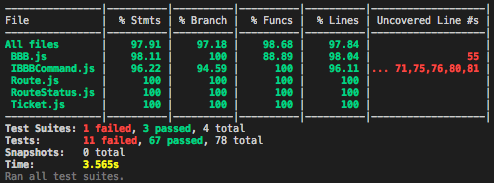
\includegraphics[width=.9\linewidth]{documentation.org.img/Iteration2_Coverage.png}
\end{center}

Using the coverage tools we checked the lines/branches that are not covered. 

\begin{center}
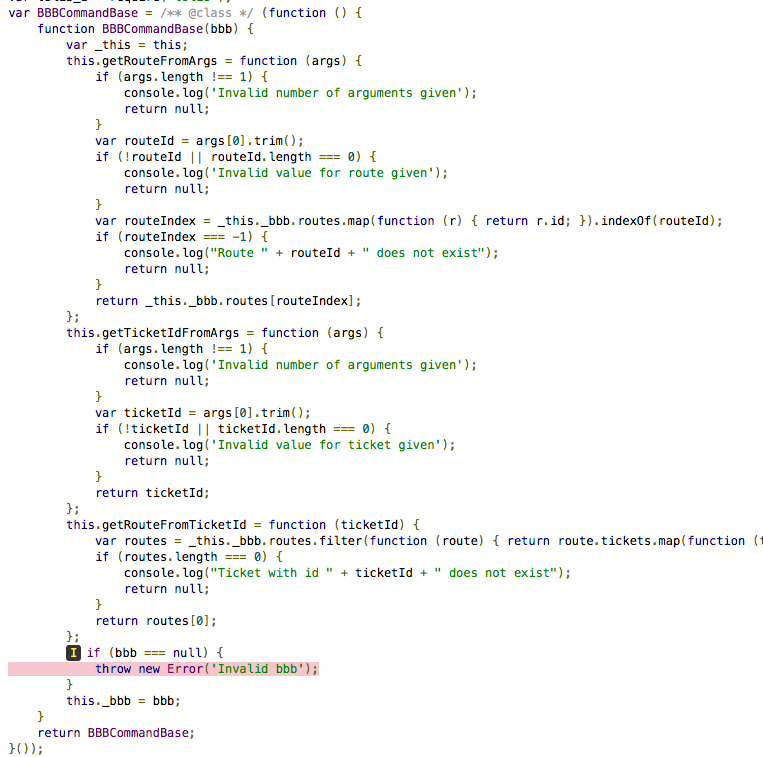
\includegraphics[width=.9\linewidth]{documentation.org.img/Iteration2_Constructor_Coverage.png}
\end{center}

For the constructor a test case is missing that tests if the initialization fails if an invalid \texttt{BBB} instance is passed.

\begin{center}
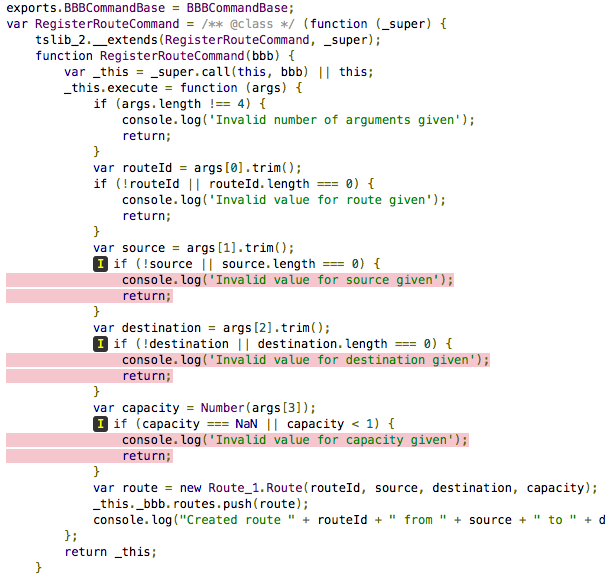
\includegraphics[width=.9\linewidth]{documentation.org.img/Iteration2_Register_Coverage.png}
\end{center}

For the \texttt{RegisterRouteCommand} the not covered lines are a result from the failing test cases. The first two if's are not covered
because an exception is thrown in TC\_RegisterRouteCommand\_4 and TC\_RegisterRouteCommand\_5 on calling trim() on a null value. Therefore
the test fails before going to the if. The third if is never true because of the failure detected in TC\_RegisterRouteCommand\_6. A 
comparison using \texttt{===} and "NaN" is always false and therefore the if branch is never taken. Thus it is not necessary to introduce 
additional test cases after fixing those three test cases.


\begin{center}
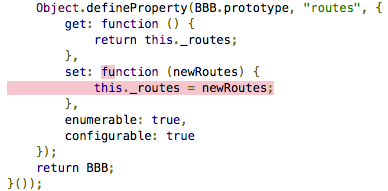
\includegraphics[width=.9\linewidth]{documentation.org.img/Iteration2_BBB_Coverage.png}
\end{center}

In the class \texttt{BBB} the setter for setting the routes is never called. Therefore, an additional test for the setter has to be created.

\subsection{Trace failures to faults}
\label{sec:org431be3e}

\subsubsection{TC\_Route\_27}
\label{sec:org3a15979}

\begin{description}
\item[{Failure}] Instead of throwing an error because of the invalid value for departed a new \texttt{Route} instance is created
\item[{Fault}] Departed is not parsed enforcing ISO\_8601 date format
\begin{center}
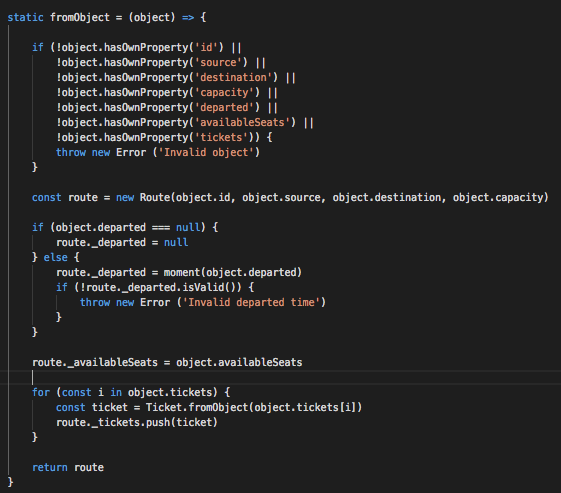
\includegraphics[width=.9\linewidth]{./Iteration2.rtfd/Pasted Graphic 8.tiff.png}
\end{center}
\item[{Fix}] Ensure that the parsing is done enfocring ISO\_8601 date format by specifying the format in the constructor
\begin{center}
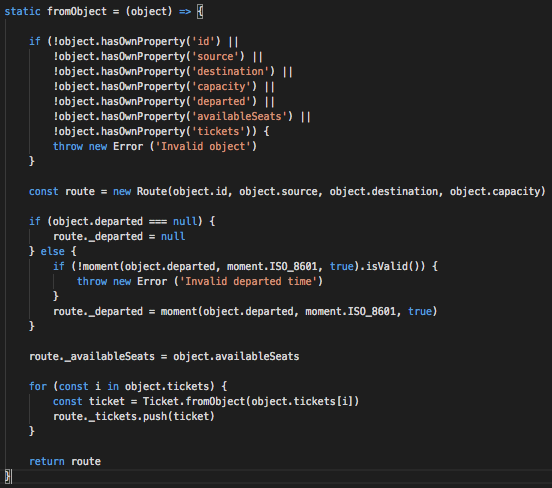
\includegraphics[width=.9\linewidth]{./Iteration2.rtfd/Pasted Graphic 7.tiff.png}
\end{center}
\end{description}

\subsubsection{TC\_RegisterRouteCommand\_4}
\label{sec:org485b9bf}

\begin{description}
\item[{Failure}] Instead of showing a meaningful error message a \texttt{TypeError} is thrown
\item[{Fault}] The method \texttt{trim()} is called on the first argument \texttt{args[0]} which is \texttt{null}
\begin{center}
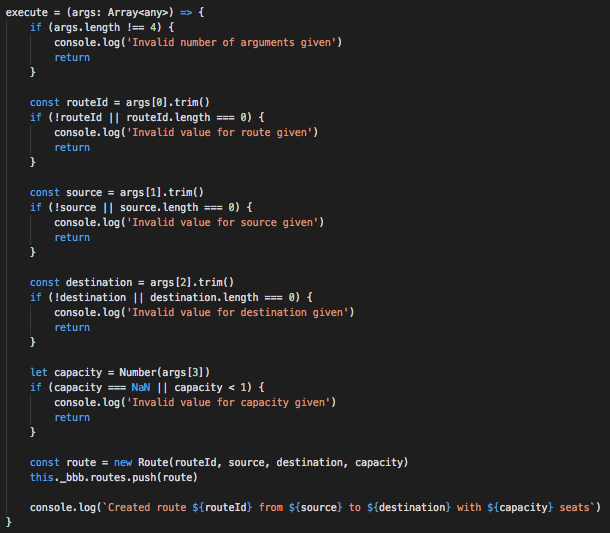
\includegraphics[width=.9\linewidth]{./Iteration3.rtfd/Pasted Graphic 7.tiff.png}
\end{center}
\item[{Fix}] Ensure that \texttt{args[1]} is not null before using the \texttt{trim()} method
\begin{center}
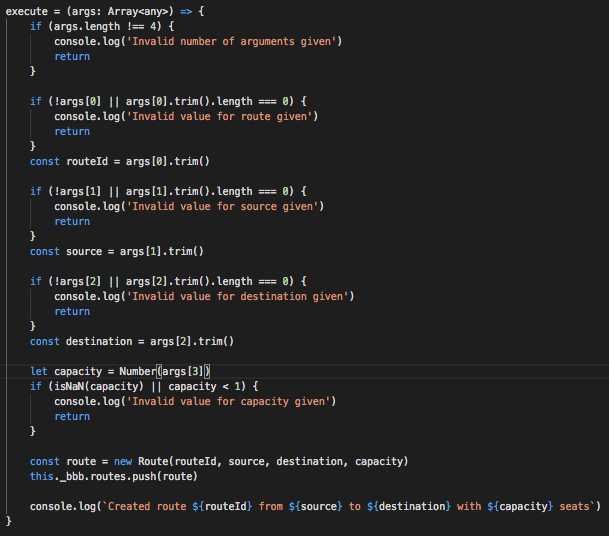
\includegraphics[width=.9\linewidth]{./Iteration3.rtfd/Pasted Graphic 14.tiff.png}
\end{center}
\end{description}

\subsubsection{TC\_RegisterRouteCommand\_5}
\label{sec:orgc4a5cbf}

The same failure and fault as in TC\_RegisterRouteCommand\_4 but with second argument \texttt{args[2]}. Is fixed the same way as TC\_RegisterRouteCommand\_4 and already shown in the previous screenshotss.

\subsubsection{TC\_RegisterRouteCommand\_6}
\label{sec:org4c22883}

\begin{description}
\item[{Failure}] Instead of showing a meaninigful error message a \texttt{RangeError} is thrown in the constructor of the \texttt{Route}
\item[{Fault}] The check if an invalid capacity has been given is done using the condition \texttt{capacity === NaN} but performing a \texttt{===} check on \texttt{NaN} always yields false
\item[{Fix}] Use the method \texttt{isNaN()} for checking for an invalid capacity (the fault and fix are also shown in the screenshots from TC\_RegisterRouteCommand\_4)
\end{description}

\subsubsection{TC\_DepartCommand\_3}
\label{sec:org3fd9eaf}

\begin{description}
\item[{Failure}] Message "Invalid value for route given" is shown instead of the message "Route R\_X does not exist"
\item[{Fault}] Actually, the observed output is correct and it is the test case that was specified wrongly
\item[{Fix}] Update the test case so that the expected output is a console message "Route R\_X does not exist" and the title states "fails for not existing route"
\end{description}

\subsubsection{TC\_BuyCommand\_3}
\label{sec:org5d59406}

\begin{description}
\item[{Failure}] Instead of showing an error message saying the tickets are sold out a \texttt{TypeError} is thrown because it is tried to access the property \texttt{id} of undefined
\item[{Fault}] After checking if the purchase of a \texttt{Ticket} was unsuccessful a return statement is missing
\begin{center}
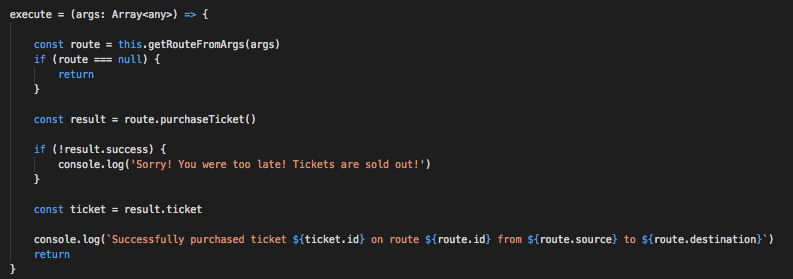
\includegraphics[width=.9\linewidth]{./Iteration3.rtfd/Pasted Graphic 9.tiff.png}
\end{center}
\item[{Fix}] Add the return statement in the case of an unsuccessful purchase attempt
\begin{center}
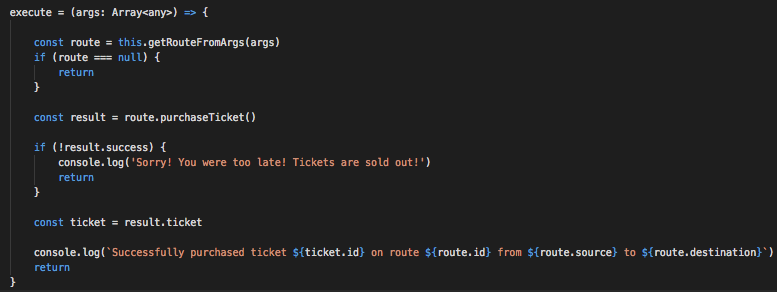
\includegraphics[width=.9\linewidth]{./Iteration3.rtfd/Pasted Graphic 16.tiff.png}
\end{center}
\end{description}

\subsubsection{TC\_CheckinCommand\_2}
\label{sec:orgc930db5}

\begin{description}
\item[{Failure}] In addition to the "Invalid number of arguments given" error message "Ticket with id null does exist" is shown
\item[{Fault}] After parsing the \texttt{ticketId} from the arguments it is not checked whether the "ticketId" is null in order to return
\begin{center}
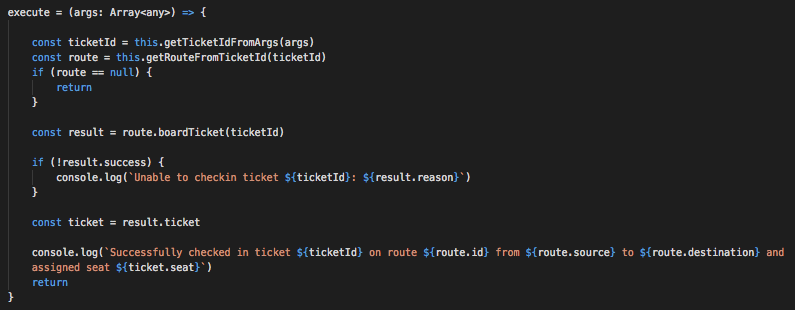
\includegraphics[width=.9\linewidth]{./Iteration3.rtfd/Pasted Graphic 10.tiff.png}
\end{center}
\item[{Fix}] Added the missing \texttt{null} check and return statement before proceeding with finding the \texttt{Route} with the \texttt{ticketId}
\end{description}

\subsubsection{TC\_CheckinCommand\_3}
\label{sec:org26daa80}

The same failure and fault as in TC\_CheckinCommand\_2. Is fixed the same way.

\subsubsection{TC\_CheckinCommand\_5}
\label{sec:org2e34fb8}

\begin{description}
\item[{Failure}] Instead of showing the expected error message saying that the ticket is already boarded a \texttt{TypeError} is thrown
\item[{Fault}] After checking if the checkin of the \texttt{Ticket} was unsuccessful a return statement is missing
\begin{center}
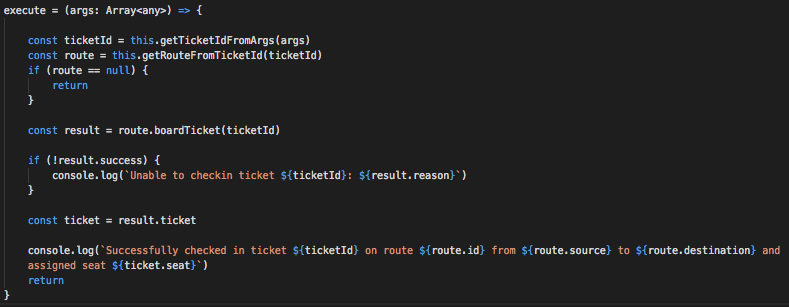
\includegraphics[width=.9\linewidth]{./Iteration3.rtfd/Pasted Graphic 11.tiff.png}
\end{center}
\item[{Fix}] Added the return statement in the cases of an unsuccessful checkin attempt
\begin{center}
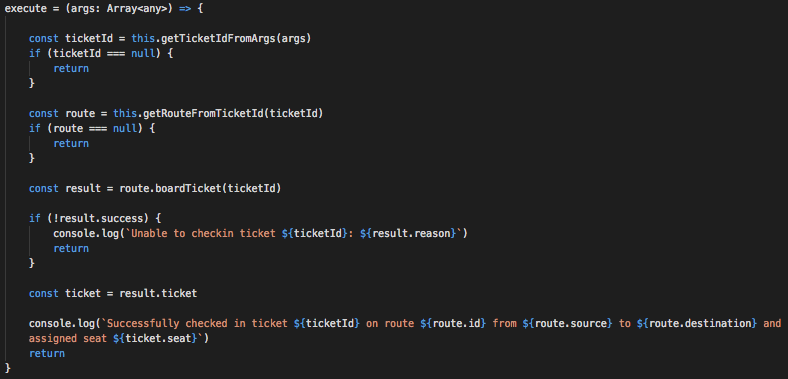
\includegraphics[width=.9\linewidth]{documentation.org.img/TC_CheckinCommand_5.png}
\end{center}
\end{description}

\subsubsection{TC\_CancelCommand\_2}
\label{sec:org1c5a87e}

\begin{description}
\item[{Failure}] In addition to the expected "Invalid number of arguments given" error message the message "Ticket with id null does not exist" is shown
\item[{Fault}] After parsing the \texttt{ticketId} from the arguments it is not checked whether the "ticketId" is null in order to return
\begin{center}
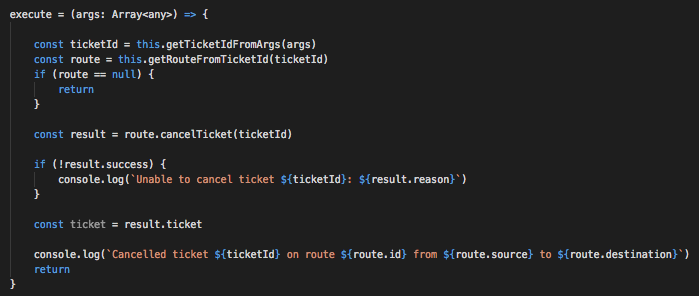
\includegraphics[width=.9\linewidth]{./Iteration3.rtfd/Pasted Graphic 12.tiff.png}
\end{center}
\item[{Fix}] Added the missing \texttt{null} check and return statement before proceeding with finding the \texttt{Route} with the \texttt{ticketId}
\begin{center}
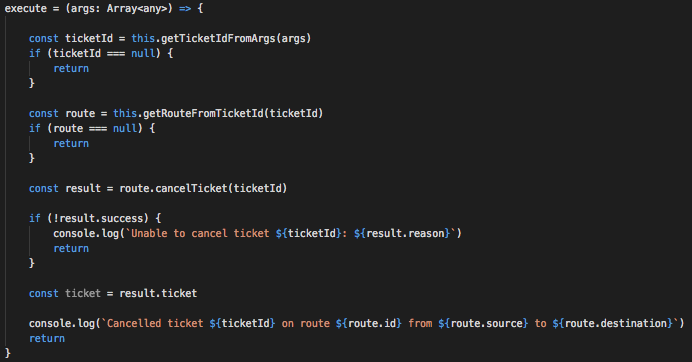
\includegraphics[width=.9\linewidth]{documentation.org.img/TC_CancelCommand_4.png}
\end{center}
\end{description}

\subsubsection{TC\_CancelCommand\_3}
\label{sec:org247bade}

The same failure and fault as in TC\_CancelCommand\_2. Is fixed the same way and already shown in the previous screenshots from TC\_CancelCommand\_2.

\subsubsection{TC\_CancelCommand\_5}
\label{sec:orgb71157d}

\begin{description}
\item[{Failure}] After showing the expected unable to cancel ticket message the message for successfully canceled the ticket is shown
\item[{Fault}] After checking if the cancelation of the \texttt{Ticket} was unsuccessful a return statement is missing (the fault is already shown in the screenshot from TC\_CancelCommand\_2)
\end{description}

\begin{description}
\item[{Fix}] Added the return statement in the cases of an unsuccessful cancel attempt (the fix is already shown in the screenshot from TC\_CancelCommand\_2)
\end{description}

\section{Iteration 3}
\label{sec:org40fc2ee}

Iteration 3 does not target a new component and only adds test cases that are missing to get full coverage.

\subsection{Specify Test Cases}
\label{sec:org5d8e024}

\subsubsection{Class IBBBCommand}
\label{sec:org452e5f6}

\begin{description}
\item[{TC\_CancelCommand\_7}] fails when initialized with invalid bbb
\begin{description}
\item[{Goal}] Test that the constructor of an \texttt{IBBBCommand} fails when initialized with an invalid \texttt{BBB}
\item[{Class}] CancelCommand
\item[{Method}] constructor
\item[{Precondition}] N/A
\item[{Input}] null
\item[{Expected Output}] Error("Invalid bbb")
\end{description}
\end{description}

\subsubsection{BBB Class}
\label{sec:orgf03050c}

\begin{description}
\item[{TC\_BBB\_8}] set routes
\begin{description}
\item[{Goals}] Test that the property \texttt{routes} can be set correctly
\item[{Class}] BBB
\item[{Method}] set route
\item[{Precondition}] routes: [\{ id: “R1”, source: “Madrid”, destination: “Toledo”, capacity: 10,  tickets: [\{id: “T\_R1\_9”, “seat”: 9, “boarded”: false\}], departed: null, availableSeats: [0, … , 8]\},
\{ id: “R2”, source: “Barcelona”, destination: “Valencia”, capacity: 10,  tickets: [], departed: null, availableSeats: [0, … , 9]\}]
\item[{Input}] routes: [\{ id: “R1”, source: “Berlin”, destination: “Toledo”, capacity: 11,  tickets: [], departed: null, availableSeats: [0, … , 9]\}]
\item[{Expected Output}] routes: [\{ id: “R1”, source: “Berlin”, destination: “Toledo”, capacity: 11,  tickets: [], departed: null, availableSeats: [0, … , 9]\}]
\end{description}
\end{description}

\subsection{Run Test Cases}
\label{sec:orgd2b81f1}

\subsubsection{Class IBBBCommand}
\label{sec:org88fdca4}

\begin{description}
\item[{TC\_CancelCommand\_7}] fails when initialized with invalid bbb
\begin{description}
\item[{Expected Output}] Error("Invalid bbb")
\item[{Observed Output}] Error("Invalid bbb")
\item[{Failure}] None
\end{description}
\end{description}

\subsubsection{Class BBB}
\label{sec:org1543c60}

\begin{description}
\item[{TC\_BBB\_8}] set routes
\begin{description}
\item[{Expected Output}] routes: [\{ id: “R1”, source: “Berlin”, destination: “Toledo”, capacity: 11,  tickets: [], departed: null, availableSeats: [0, … , 9]\}]
\item[{Observed Output}] routes: [\{ id: “R1”, source: “Berlin”, destination: “Toledo”, capacity: 11,  tickets: [], departed: null, availableSeats: [0, … , 9]\}]
\item[{Failure}] None
\end{description}
\end{description}

\subsection{Check Coverage}
\label{sec:orgc57f24f}

\begin{center}
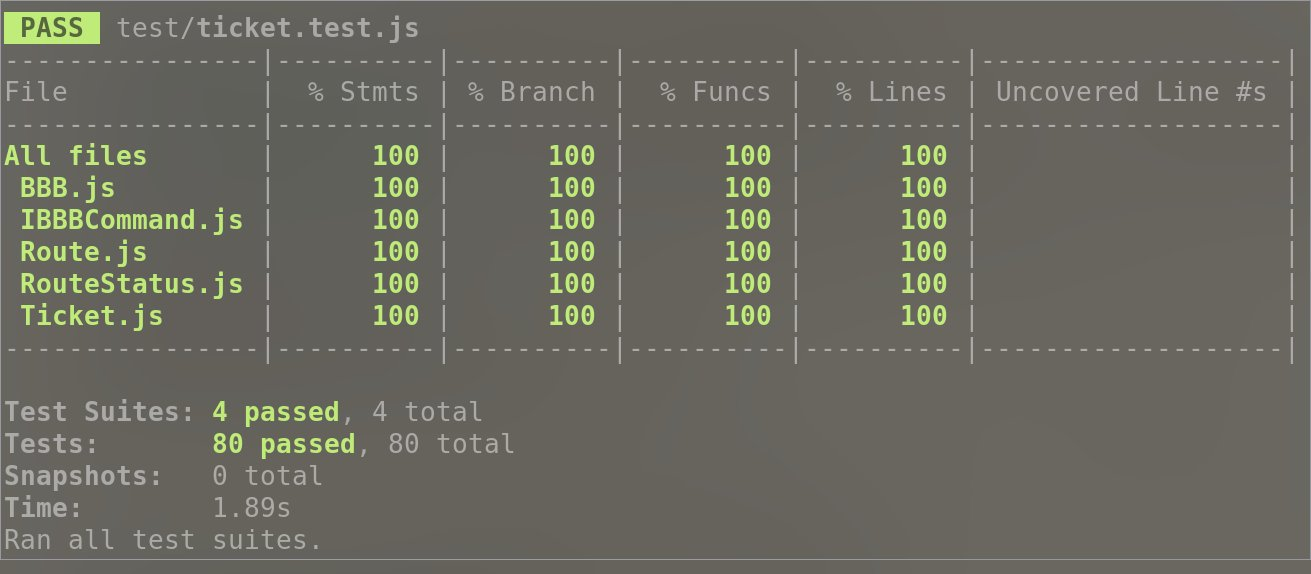
\includegraphics[width=.9\linewidth]{documentation.org.img/org_20181130_185109_LYvGqi.jpg}
\end{center}

We reached 100\% branch coverage for all files without any tests failing. Therefore the white box assignment is completed. Since we used a unit test approach,
we tested each component of the application individually and isolated. Even though we reached the full branch coverage which was the aim of this assignment, we 
would usually also implement integration tests to ensure that the application works correctly when all components are used jointly. 
\end{document}
